    %%%%%%%% ICML 2024 EXAMPLE LATEX SUBMISSION FILE %%%%%%%%%%%%%%%%%
\PassOptionsToPackage{dvipsnames,table}{xcolor}
\documentclass{article}

% Recommended, but optional, packages for figures and better typesetting:
\usepackage{microtype}
\usepackage{graphicx}
\usepackage{subfig}
\usepackage{booktabs} % for professional tables

% hyperref makes hyperlinks in the resulting PDF.
% If your build breaks (sometimes temporarily if a hyperlink spans a page)
% please comment out the following usepackage line and replace
% \usepackage{icml2024} with \usepackage[nohyperref]{icml2024} above.
\usepackage{hyperref}


% Attempt to make hyperref and algorithmic work together better:
\newcommand{\theHalgorithm}{\arabic{algorithm}}

% Use the following line for the initial blind version submitted for review:
% \usepackage{icml2024}

% If accepted, instead use the following line for the camera-ready submission:
\usepackage[accepted]{icml2024}

% For theorems and such
\usepackage{amsmath}
\usepackage{amssymb}
\usepackage{mathtools}
\usepackage{amsthm}

% if you use cleveref..
\usepackage[capitalize,noabbrev]{cleveref}

%%%%%%%%%%%%%%%%%%%%%%%%%%%%%%%%
% THEOREMS
%%%%%%%%%%%%%%%%%%%%%%%%%%%%%%%%
\theoremstyle{plain}
\newtheorem{theorem}{Theorem}[section]
\newtheorem{proposition}[theorem]{Proposition}
\newtheorem{lemma}[theorem]{Lemma}
\newtheorem{corollary}[theorem]{Corollary}
\theoremstyle{definition}
\newtheorem{definition}[theorem]{Definition}
\newtheorem{assumption}[theorem]{Assumption}
\theoremstyle{remark}
\newtheorem{remark}[theorem]{Remark}

% Todonotes is useful during development; simply uncomment the next line
%    and comment out the line below the next line to turn off comments
%\usepackage[disable,textsize=tiny]{todonotes}
\usepackage[textsize=tiny]{todonotes}


% Add my packages starting from here

% Standard package includes
\usepackage{times}
\usepackage{latexsym}
\usepackage{natbib}

% For proper rendering and hyphenation of words containing Latin characters (including in bib files)
\usepackage[T1]{fontenc}
% For Vietnamese characters
% \usepackage[T5]{fontenc}
% See https://www.latex-project.org/help/documentation/encguide.pdf for other character sets

% This assumes your files are encoded as UTF8
\usepackage[utf8]{inputenc}

% This is not strictly necessary, and may be commented out,
% but it will improve the layout of the manuscript,
% and will typically save some space.
\usepackage{microtype}
\usepackage{url}
\usepackage{amsmath,amsfonts,amssymb}

\usepackage{multirow}
% \DeclareMathOperator*{\argmax}{arg\,max}
% \DeclareMathOperator*{\argmin}{arg\,min}
\usepackage{mathrsfs}
\usepackage{algorithm}
\usepackage{algorithmic}
\usepackage{graphicx}
\usepackage{bbm}
\usepackage{wrapfig,lipsum,booktabs}
\usepackage{pifont}
\usepackage{placeins}
\usepackage[normalem]{ulem}

\makeatletter
\patchcmd{\BR@backref}{\newblock}{\newblock(page~}{}{}
\patchcmd{\BR@backref}{\par}{)\par}{}{}
\makeatother

\useunder{\uline}{\ul}{}
\newcommand{\cmark}{\ding{51}}
\newcommand{\xmark}{\ding{55}}

\newcommand{{\ourmethod}}{APT}
\newcommand{{\ourarch}}{APT adapter}
% \newcommand{\ourarchabbr}{$\mathcal{E}\text{Adapter}$}
\newcommand{\ourarchabbr}{APT adapter}
\newcommand{\tableindent}{~~~~}
\newcommand{\lmabbr}{LM}
\newcommand{\pruningabbr}{SP}
% \newcommand\todo[1]{\textit{\textcolor{purple}{[TODO] #1}}}

\newcommand{\draftonly}[1]{#1} 
% Uncomment for submission
% \renewcommand{\draftonly}[1]{}
\newcommand{\draftcomment}[3]{\draftonly{{\textcolor{#3}{[\small \textbf{\textsc{#2}: #1}]}}}}
\newcommand{\qq}[1]{\draftcomment{#1}{QC}{teal}}
\newcommand{\bowen}[1]{\draftcomment{#1}{BW}{magenta}}
\newcommand{\hanna}[1]{\draftcomment{#1}{HH}{orange}}


% The \icmltitle you define below is probably too long as a header.
% Therefore, a short form for the running title is supplied here:
\icmltitlerunning{APT: Adaptive Pruning and Tuning Pretrained Language Models for Efficient Training and Inference}

\begin{document}

\twocolumn[
\icmltitle{APT: Adaptive Pruning and Tuning Pretrained Language Models for \\Efficient Training and Inference}

% It is OKAY to include author information, even for blind
% submissions: the style file will automatically remove it for you
% unless you've provided the [accepted] option to the icml2024
% package.

% List of affiliations: The first argument should be a (short)
% identifier you will use later to specify author affiliations
% Academic affiliations should list Department, University, City, Region, Country
% Industry affiliations should list Company, City, Region, Country

% You can specify symbols, otherwise they are numbered in order.
% Ideally, you should not use this facility. Affiliations will be numbered
% in order of appearance and this is the preferred way.
\icmlsetsymbol{equal}{*}

\begin{icmlauthorlist}
\icmlauthor{Bowen Zhao}{xxx}
\icmlauthor{Hannaneh Hajishirzi}{xxx,yyy}
\icmlauthor{Qingqing Cao$^*$}{zzz}
% \icmlauthor{Firstname4 Lastname4}{sch}
% \icmlauthor{Firstname5 Lastname5}{yyy}
% \icmlauthor{Firstname6 Lastname6}{sch,yyy,comp}
% \icmlauthor{Firstname7 Lastname7}{comp}
% %\icmlauthor{}{sch}
% \icmlauthor{Firstname8 Lastname8}{sch}
% \icmlauthor{Firstname8 Lastname8}{yyy,comp}
%\icmlauthor{}{sch}
%\icmlauthor{}{sch}
\end{icmlauthorlist}

\icmlaffiliation{xxx}{University of Washington}
\icmlaffiliation{yyy}{Allen Institute for Artificial Intelligence}
\icmlaffiliation{zzz}{$^*$Apple, work done at the University of Washington}
% \icmlaffiliation{sch}{School of ZZZ, Institute of WWW, Location, Country}

\icmlcorrespondingauthor{Bowen Zhao}{bowen98@uw.edu}
\icmlcorrespondingauthor{Qingqing Cao}{qicao@apple.com}

% You may provide any keywords that you
% find helpful for describing your paper; these are used to populate
% the "keywords" metadata in the PDF but will not be shown in the document
\icmlkeywords{Machine Learning, ICML}

\vskip 0.3in
]

% this must go after the closing bracket ] following \twocolumn[ ...

% This command actually creates the footnote in the first column
% listing the affiliations and the copyright notice.
% The command takes one argument, which is text to display at the start of the footnote.
% The \icmlEqualContribution command is standard text for equal contribution.
% Remove it (just {}) if you do not need this facility.

\printAffiliationsAndNotice{}  % leave blank if no need to mention equal contribution
% \printAffiliationsAndNotice{\icmlEqualContribution} % otherwise use the standard text.

\begin{abstract}
Fine-tuning and inference with large Language Models~({\lmabbr}) are generally known to be expensive. 
Parameter-efficient fine-tuning over pretrained LMs reduces training memory by updating a small number of {\lmabbr} parameters but does not improve inference efficiency. Structured pruning improves {\lmabbr} inference efficiency by removing consistent parameter blocks, yet often increases training memory and time. To improve both training and inference efficiency, we introduce {\ourmethod} that adaptively {\it prunes} and {\it tunes} parameters for the {\lmabbr}s. 
At the early stage of fine-tuning, {\ourmethod} dynamically adds {\it salient} tuning parameters for fast and accurate convergence while discarding unimportant parameters for efficiency.
Compared to baselines, our experiments show that {\ourmethod} maintains up to 98\% task performance when pruning 60\% of the parameters in RoBERTa and T5 models. APT also preserves 86.4\% of LLaMA models' performance with 70\% parameters remaining. Furthermore, {\ourmethod} speeds up LMs' fine-tuning by up to 8$\times$ and reduces large {\lmabbr}s' memory training footprint by up to 70\%. Our code and models are publicly available at \url{https://github.com/ROIM1998/APT}.
\end{abstract}


\section{Introduction}
%pretrained Language models ({\lmabbr}s) have shown strong performance on various natural language processing tasks~\citep{devlin-etal-2019-bert,liu2019roberta,raffel2020exploring}, while large language models (LLMs)~\citep{brown2020language,zhang2022opt} with more parameters show their reasoning and generalization capabilities outperforming small {\lmabbr}s~\citep{kaplan2020scaling}. 
% \hanna{please dont' use PLM and LLM acronyms... just use LMs and add pretrained or large adjectives if needed.} 
% \hanna{first sentence is not needed} 
Fine-tuning language models (LMs)~\citep{devlin-etal-2019-bert,liu2019roberta,raffel2020exploring} is an essential paradigm to adapt them to downstream tasks~\citep{mishra-etal-2022-cross,wang-etal-2022-super}. Increasing the parameter scale of LMs improves model performance~\citep{kaplan2020scaling}, but incurs significant training and inference costs.  
%However, as the parameter size of {\lmabbr} increases, both training and inference efficiency bottlenecks hinder the practicality of {\lmabbr}'s wide usage. 
For instance, a 13B LLaMA model~\citep{touvron2023llama} costs about 100GB memory for fine-tuning and 30GB for inference with float16 datatype. 
It is important to improve the training and inference efficiency of {\lmabbr} for practical applications.

\begin{figure}[t!]
    \centering
    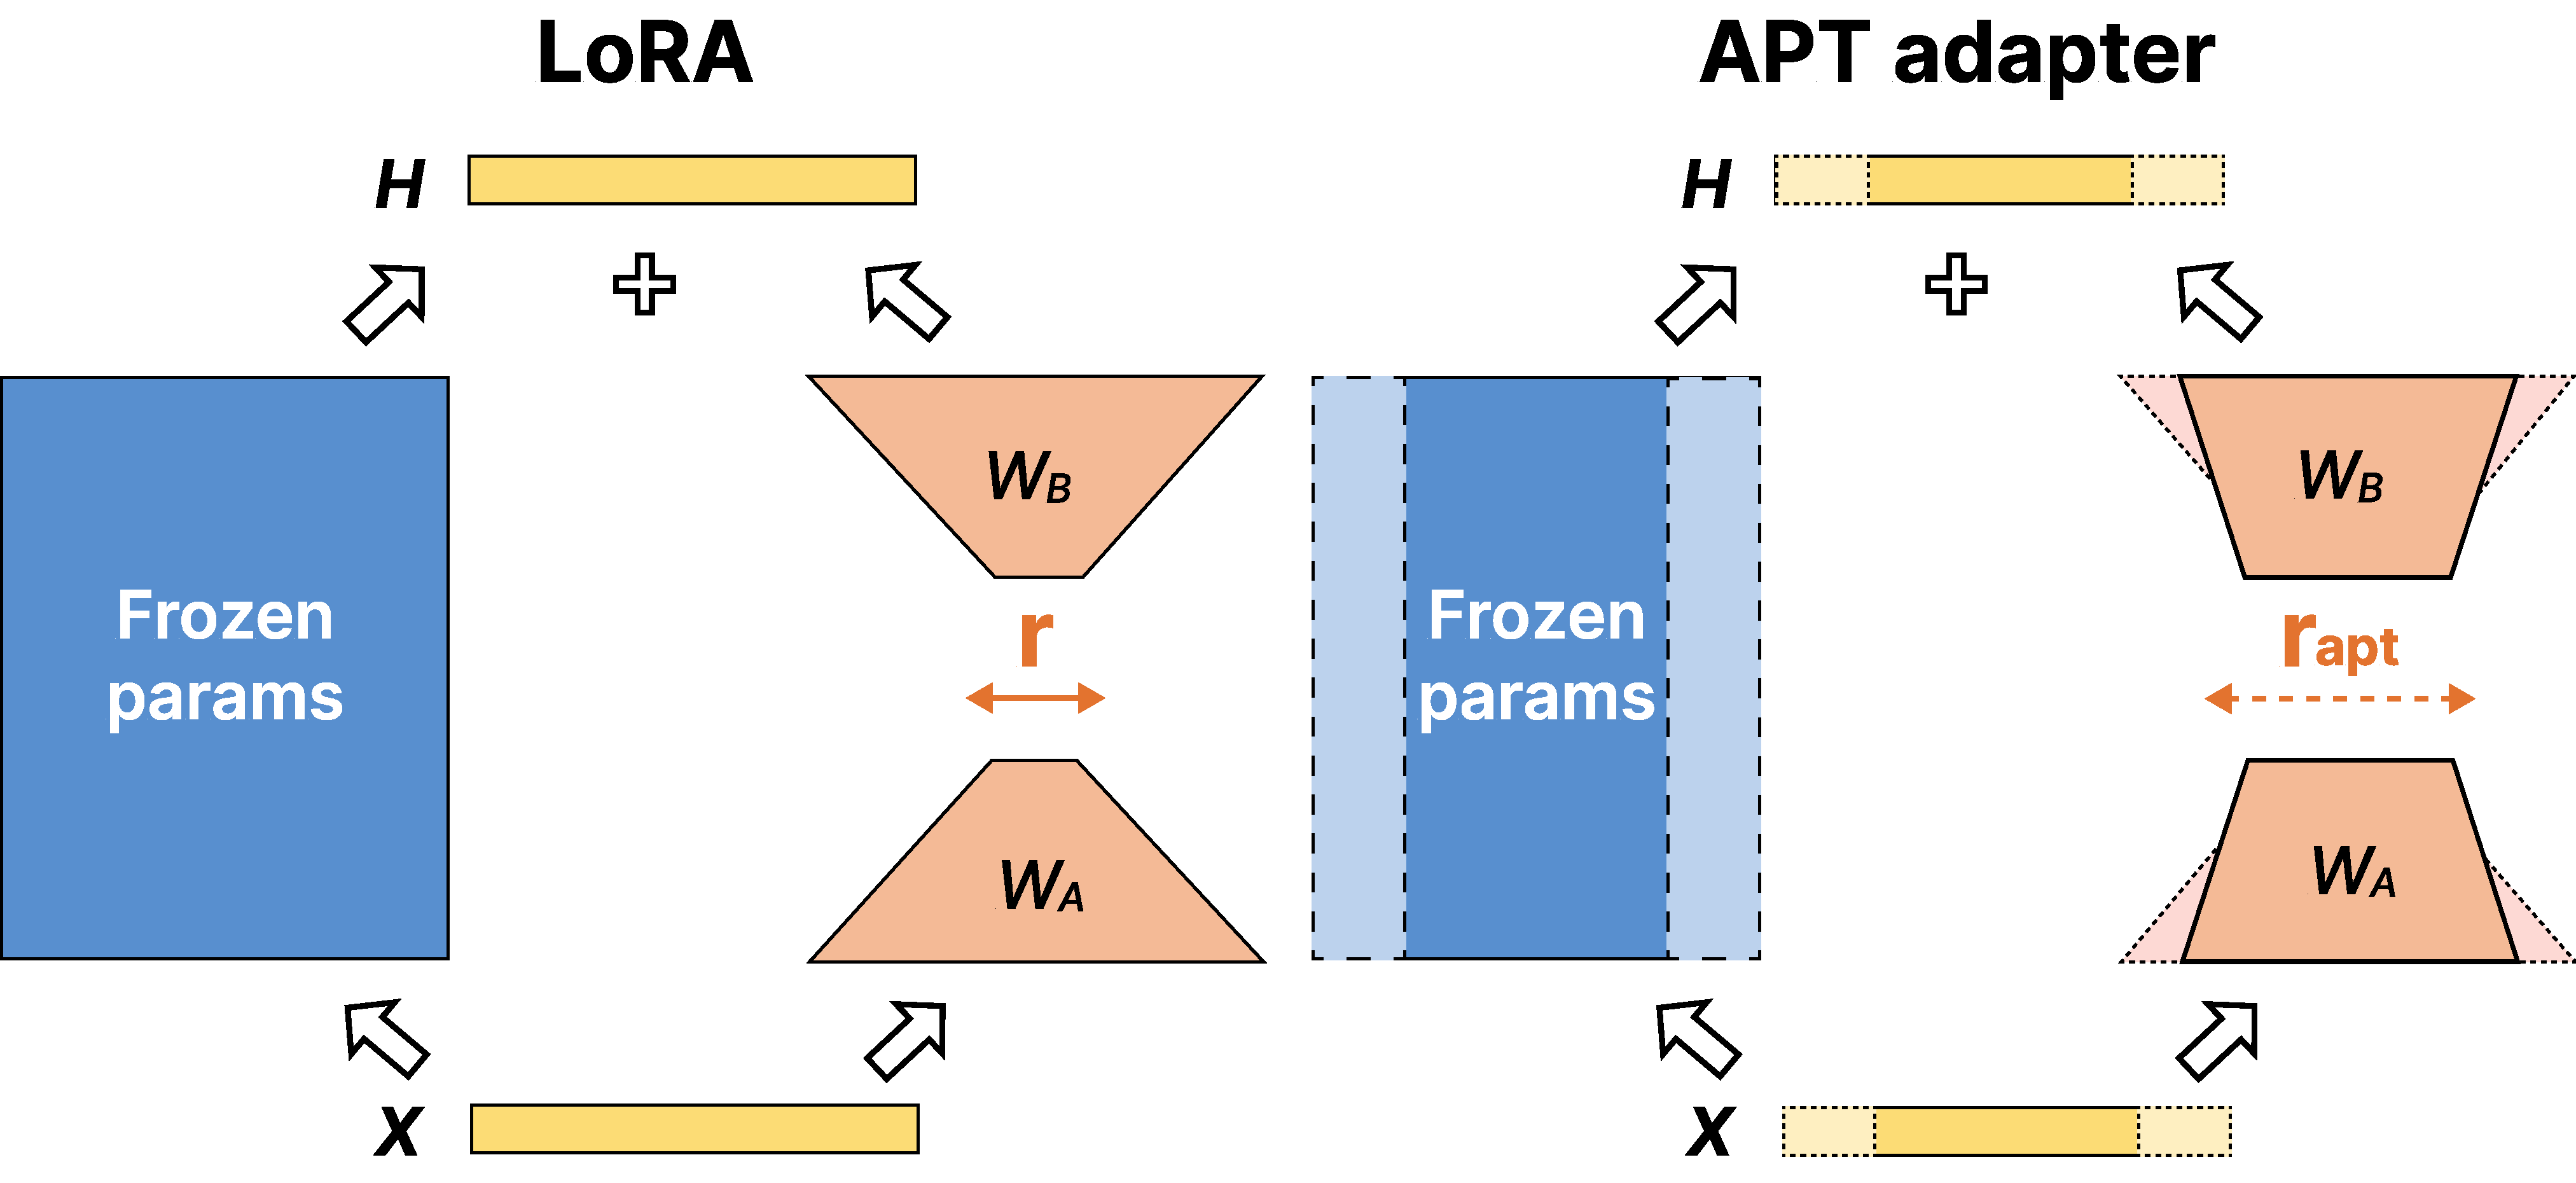
\includegraphics[width=0.9\linewidth]{figures/teaser_figure_revised.pdf}
\caption{{\ourmethod} provides both training and inference efficiency benefits by pruning and tuning pretrained LM parameters adaptively via the \textbf{{\ourmethod} adapter}. We dynamically adjust (add/reduce) {\ourmethod} adapter input/output dimensions and the rank ($r_{\text{apt}}$). Reducing adapter dimensions prunes frozen parameters, making training and inference faster and more memory-efficient. Adding adapter ranks helps recover the pruned {\lmabbr}'s task performance. In contrast, existing adapters like LoRA allow efficient training but do not provide inference efficiency since the model size is not reduced.}
    \label{fig:teaser}
    \vspace{-15pt}
\end{figure}


% \qq{We can first discuss efficient training, PEFT methods, their main benefits are memory reduction, no speedup etc. Deploying PEFT trained models do not directly provide inference efficiency, so we discuss inference efficiency methods like quantization, pruning etc. And those inference methods requires full fine-tuning, and naive solutions like applying PEFT+quant/pruning do not work out of the box. Then you describe why it does not work, and what are the challenges (you already have something about this in the next paragraph).}

% Please add the following required packages to your document preamble:
% \usepackage{booktabs}
\begin{table*}[t!]
\centering
\small
\begin{tabular}{@{}ll|cc|cc|cc@{}}
\toprule
\multicolumn{2}{l|}{\multirow{2}{*}{Method}} & \multirow{2}{*}{$\mathcal{A}_{\text{P}}$} & \multirow{2}{*}{$\mathcal{A}_{\text{T}}$} & \multicolumn{2}{c|}{Training}                                             & \multicolumn{2}{c}{Inference}                                                        \\
\multicolumn{2}{l|}{}                        &                     &                     & T                                          & M                         & T                                                  & M                          \\ \midrule
\multirow{3}{*}{PEFT}       & Adapter~\citep{Pfeiffer2020AdapterFusionNT}        & \xmark              & \xmark              & \color{red}$\Uparrow_{\text{High}}$ & \color{ForestGreen}$\Downarrow_{\text{Low}}$ & \color{red}$\Uparrow_{\text{Low}}$                              & \color{red}$\Uparrow_{\text{Low}}$      \\
                            & LoRA~\citep{hu_lora_2021}           & \xmark              & \xmark              & \color{red}$\Uparrow_{\text{High}}$ & \color{ForestGreen}$\Downarrow_{\text{Low}}$ & \textbf{=}                                         & \textbf{=}                 \\
                            & AdaLoRA~\citep{zhang2023adaptive}        & \xmark              & \cmark              & \color{red}$\Uparrow_{\text{High}}$ & \color{ForestGreen}$\Downarrow_{\text{Low}}$ & \textbf{=}                                         & \textbf{=}                 \\ \midrule
\multirow{4}{*}{Pruning}    & MvP~\citep{sanh_movement_2020}            & \xmark              & \xmark              & \color{red}$\Uparrow_{\text{High}}$ & \color{red}$\Uparrow_{\text{Low}}$     & \color{ForestGreen}$\Downarrow_{\text{Low}}$                         & \color{ForestGreen}$\Downarrow_{\text{Low}}$ \\
                            & BMP~\citep{lagunas_block_2021}            & \xmark              & \xmark              & \color{red}$\Uparrow_{\text{High}}$ & \color{red}$\Uparrow_{\text{Low}}$     & \color{ForestGreen}$\Downarrow_{\text{High}}$ & \color{ForestGreen}$\Downarrow_{\text{Low}}$  \\
                            & CoFi~\citep{xia_structured_2022}           & \xmark              & \xmark              & \color{red}$\Uparrow_{\text{High}}$ & \color{red}$\Uparrow_{\text{Low}}$     & \color{ForestGreen}$\Downarrow_{\text{High}}$ & \color{ForestGreen}$\Downarrow_{\text{Low}}$  \\
                            & MT~\citep{kwon_fast_2022}             & \xmark              & \xmark              & \textbf{=}                                 & \textbf{=}                & \color{ForestGreen}$\Downarrow_{\text{High}}$ & \color{ForestGreen}$\Downarrow_{\text{Low}}$  \\ \midrule
\multirow{3}{*}{Combined}   & SPA~\citep{hedegaard_structured_2022}            & \xmark              & \xmark              & \color{red}$\Uparrow_{\text{High}}$ & \color{red}$\Uparrow_{\text{Low}}$     & \color{ForestGreen}$\Downarrow_{\text{High}}$ & \color{ForestGreen}$\Downarrow_{\text{Low}}$  \\
                            & LRP~\citep{zhang2023pruning}            & \xmark              & \xmark              & \color{red}$\Uparrow_{\text{High}}$ & \color{ForestGreen}$\Downarrow_{\text{Low}}$ & \color{ForestGreen}$\Downarrow_{\text{High}}$ & \color{ForestGreen}$\Downarrow_{\text{Low}}$  \\
                            & \textbf{\ourmethod} (ours)   & \cmark              & \cmark              & \color{red}$\Uparrow_{\text{Low}}$                      & \color{ForestGreen}$\Downarrow_{\text{Low}}$ & \color{ForestGreen}$\Downarrow_{\text{High}}$ & \color{ForestGreen}$\Downarrow_{\text{Low}}$  \\ \bottomrule
\end{tabular}
\caption{Efficiency comparison of existing methods and APT. $\mathcal{A}_{\text{P}}$ stands for adaptive pruning and $\mathcal{A}_{\text{T}}$ for adaptive tuning, where the total and tuning parameter sizes are dynamically adjusted. We measure efficiency using training converge time, inference time (T), and peak memory (M). Symbols {\color{red}$\Uparrow$} and {\color{ForestGreen}$\Downarrow$} indicate increased and decreased costs, respectively, while \textbf{=} signifies no change in cost. The terms ``low'' and ``high'' qualify the extent of cost variations.} 
\label{tab:preliminary-summary}
\vspace{-15pt}
\end{table*}

Parameter-efficient fine-tuning methods (PEFT, summarized in \cref{tab:preliminary-summary})~\citep{houlsby2019parameter,li2021prefix} reduce the memory consumption of LM fine-tuning via updating a small number of parameters. However, PEFT models do not improve inference efficiency because the {\lmabbr} size remains the same or even increases after fine-tuning. For instance, LoRA~\citep{hu_lora_2021} tunes low-rank decomposed linear layers parallel to frozen parameters to reduce training memory but takes longer to converge~\citep{ding2023parameter}.
On the other hand, structured pruning~\cite{kwon_fast_2022,xia_structured_2022,ma2023llm} improves inference efficiency by removing blocks of parameters such as attention heads and feed-forward neurons in Transformer {\lmabbr}s, showing more inference speedup than sparse unstructured pruning methods~\citep{Han2015DeepCC,han2015learning,sanh_movement_2020}. However, training pruned {\lmabbr}s takes extra time to converge and incurs high memory, substantially diminishing LMs' accessibility in usage scenarios with limited computational resources.

Integrating structured pruning and PEFT could increase both training and inference efficiency. 
However, existing research~\citep{zhao2023cpet} indicates that combining PEFT and structured pruning, such as applying structured pruning over LoRA-tuned models, causes noticeable performance loss and extra training costs. It remains challenging to prune {\lmabbr}s accurately using limited training resources.

In this paper, we develop an efficient fine-tuning approach named {\ourmethod} that \textbf{A}daptively selects model parameters for \textbf{P}runing and fine-\textbf{T}uning. {\ourmethod} combines the benefits of PEFT and structured pruning to make fine-tuning and inference more efficient. Our intuition is that pre-trained {\lmabbr} parameters contain general knowledge, but their importance to downstream tasks varies. Therefore, we can remove the parameters irrelevant to the fine-tuning task in the early training stage. Early-removing these parameters improves training and inference efficiency while not substantially hurting model accuracy~\citep{frankle2021pruning,Shen_2022_CVPR,zhang2023emergent}. Meanwhile, continuously adding more parameters for fine-tuning can improve LM performance because task-specific skills live in a subset of {\lmabbr} parameters~\citep{wang-etal-2022-finding-skill,panigrahi2023task}. 

More specifically, {\ourmethod} learns the pruning masks via an outlier-aware salience scoring function to remove irrelevant {\lmabbr} parameter blocks and adds more tuning parameters during fine-tuning according to tuning layer importance. To make training more efficient, the salience scoring function is lightweight and causes little runtime and memory overhead. Combined with our self-distillation technique that shares teacher and student parameters, {\ourmethod} can accurately prune an {\lmabbr} with less training time and lower memory usage.
% {\ourmethod} is designed by observing these intuitions: a) 



% We design our {\ourarch} architecture in {\ourmethod} framework that can adaptively increase salient parameters to be tuned while pruning redundant or unimportant parameters based on the efficient outlier-aware salience scores derived from {\lmabbr} hidden states, letting {\lmabbr} training converge fast and accurate in low-memory settings.
% \qq{I remember you have a way to view the tuning and pruning parameters together and have a technique to decide which to prune and tune, say it specifically here, because "jointly identifies" is unclear how you do it.} \qq{this is vague, you can highlight the benefits or our methods clearly, like some speedup keep accuracy comparable etc.}
% \qq{prefer to avoid `novel', people can tell if your methods are novel or not} 
% \hanna{the name elastic.. does not matter here much. YOu need to describe the metho and explain what it does rather than we build our .. method}
% \qq{compress the two techqniues into two key ideas, briefly explain how to do it and why it can work or what benefits it brings}

% We conduct comprehensive experiments on various tasks with different {\lmabbr} backbones.
% \qq{mention our method benefits both small scale and large scale models, some key numbers like xx speedup, save xx memory etc.} \todo{Two sets of results: faster pruning small models and less memory pruning large {\lmabbr}s}
% \qq{what about other baselines, you could say the best results compared to baselines (it's not LoRA, should be lora+pruning?), also did you explain or define LoRA before (if not, better mention it when you talk about PEFT), otherwise it feels abrupt to suddenly mention LoRA}
% \qq{make it consistent between intro and abstract}
Experimental results show that {\ourmethod} prunes RoBERTa and T5 base models 8$\times$ faster than the LoRA plus pruning baseline while reaching 98.0\% performance with 2.4 $\times$ speedup and 78.1\% memory consumption during inference. When pruning large {\lmabbr}s like LLaMA, {\ourmethod} costs only 30\% memory compared to the state-of-the-art pruning method and still maintains 86.4\% performance with 70\% parameters. Our ablation study in \cref{sec:ablation} indicates the effectiveness of adaptive pruning and tuning. It also demonstrates that efficient distillation with {\ourarchabbr} substantially recovers small {\lmabbr}s' performance while outlier-aware salience scoring prunes large {\lmabbr}s more accurately. Our analysis in \cref{sec:analysis} demonstrates that controlled adaptive tuning with early pruning during fine-tuning improves {\lmabbr} end-task accuracy better with less training time and memory costs.
% \qq{also need to add a few key ablation results, showing that each of the proposed methods works effectively either improving efficiency or maintaining accuracy etc.}
\section{Related Works} 

\subsection{Parameter-efficient Fine-tuning (PEFT)}
% \qq{you need to explicitly discuss at least LoRA, then explain its drawbacks compared to our method (since we build on top of LoRA), our method uses adaptive parameters xxx. Also, what about AdaLoRA>}
PEFT methods aim to tune {\lmabbr}s with limited resources by updating a small number of parameters~\citep{lialin2023scaling}, mainly falling into three categories: selective, additive, and dynamic. Selective methods focus on tuning a subset of parameters in {\lmabbr}s with pre-defined rules~\citep{ben-zaken-etal-2022-bitfit} or importance metrics~\citep{sung2021training,guo-etal-2021-parameter}. Additive methods tune injected layer modules~\citep{houlsby2019parameter,Pfeiffer2020AdapterFusionNT} or embeddings~\citep{lester-etal-2021-power,li2021prefix}. For example, LoRA~\citep{hu_lora_2021} tunes low-rank decomposed layers to avoid inference cost overhead. However, LoRA keeps the tuning layer shapes static without dynamic adjustments. Dynamic methods~\citep{he-etal-2022-sparseadapter} adjust tuning parameters during training. For instance, AdaLoRA~\citep{zhang2023adaptive} gradually reduces tuning parameters but does not benefit inference efficiency. Compared to these methods, {\ourmethod} adaptively adjusts the pruning and tuning parameters simultaneously, improving training and inference efficiency.
% In the meantime, even though IncreLoRA~\citep{zhang2023increlora} reverses the allocation strategy to increase LoRA parameters during training, the SVD decomposition used in it would incur training time and memory overhead compared to LoRA. 
% Furthermore, using PEFT alone does not bring inference efficiency gains, and adding non-linear modules for tuning even costs inference speed degradation. 
% \qq{also discuss their inference is not faster than fine-tuned models, some adapter methods (adding parameters) are even slower, maybe group these PEFT methods into three categories: only tuning parameters, add tunable parameters, dynamically allocate parameters (are they slower in inference too?). }
% \bowen{Sure. How about just two: static additive methods except LoRA bring inference efficiency degradation, and dynamic selective methods cost peak memory overhead at the start of the training. BitFit is a kind of ``corner case'' here which is a static selective method.}

\subsection{Model Compression}
% \qq{make it two paragraphs, like quantization and pruning, explain each}
% \qq{change to pruning and quantization (Or just model compression because next section you say combining compression and PEFT)? Unstructured pruning is not our focus because they do not provide speedup (need specialized software/hardware). Also need to briefly discuss quantization (some quantization does provide inference speedup?) } \bowen{Edited it as briefly talking about quantization, then pruning, and specifically for structured pruning, but I think it looks too long right now. }
% \hanna{1) are these models: lora + pruning or lora + quantization? does it mean lora + sparse pruning exists, but here apt is lora + structured pruning? what does it mean that structured pruning provides ubiquitous inference speedup?  }
% Quantization converts parameters to low-bit datatypes for memory reduction. QLoRA~\citep{dettmers2023qlora} quantizes {\lmabbr} during fine-tuning while AWQ~\citep{lin2023awq} conducts fast quantization after fine-tuning, yet the speedup gain of quantization methods needs specific framework support, which is not as ubiquitous and effective as structured pruning.
Model compression methods like quantization and pruning boost inference efficiency. Quantization aims to reduce {\lmabbr}s' memory consumption via converting parameters to low-bit data types~\citep{Frantar2022GPTQAP,Dettmers2022LLMint88M,lin2023awq}. However, despite reducing {\lmabbr}'s memory consumption, the speedup benefits of quantization require specific framework support, which limits their adaptability.
Pruning~\citep{LeCun1989OptimalBD,Han2015DeepCC,frankle2018lottery,xu2021rethinking} aims to discard unimportant parameters in {\lmabbr}s for inference efficiency. Unstructured pruning~\citep{sanh_movement_2020} prunes sparse parameters in {\lmabbr}s, which requires dedicated hardware support for efficiency improvements. Meanwhile, structured pruning~\citep{lagunas_block_2021,xia_structured_2022} prunes consistent blocks in transformer layers (MHA heads, FFN neurons, and model dimensions) for ubiquitous inference efficiency gains. Such pruning often uses knowledge distillation~\citep{Hinton2015DistillingTK}, which causes more training costs. Post-training pruning~\citep{kwon_fast_2022,Frantar2023SparseGPTML} aims to prune fine-tuned models with limited extra costs but requires initialization from fully fine-tuned models. Moreover, task-agnostic pruning~\citep{sun2023simple,ma2023llm} cannot achieve on-par performance with task-specific pruning.

\subsection{Combining Compression and PEFT}
Combining model compression and PEFT might achieve both training and inference efficiency improvements: QLoRA~\citep{dettmers2023qlora} and QA-LoRA~\citep{xu2023qa} bring quantization and LoRA together for large {\lmabbr} tuning. SPA~\citep{hedegaard_structured_2022} combines structured pruning and Compacter~\citep{karimi2021compacter}, yet suffers substantial performance loss. CPET~\citep{zhao2023cpet} leverages different task-agnostic model compression methods together with LoRA and knowledge distillation, but the performance loss becomes notable specifically when structured pruning is applied. PST~\citep{ijcai2022p586} and LRP~\citep{zhang2023pruning} also explored the combination of LoRA and pruning, yet their performance degradations are also substantial because their tuning parameters are static.
% \qq{why they are worse, any one sentence explanation will be helpful, another drawback for those unstructured pruning is they need dedicated hardware/framework to support inference speedup}
In contrast, {\ourmethod} identifies tuning and pruning parameters based on their salience in fine-tuning, which can improve training and inference efficiency under a new paradigm with minimal performance loss. 
% \qq{use is not a good word, something like considering tuning and pruning from parameters capacity view xxx, improving both training and inference in a new way xxx},

% We propose our {\ourarchabbr} architecture for adaptable block tuning and pruning while training transformer-based {\lmabbr}s. Based on this architecture, we use Fisher information as the scoring function for block tuning and pruning with self-distillation objectives for efficient and accurate training. Meanwhile, we develop our parameter scheduler that controls the training process, which would gradually discard non-salient parameters during the training stage and re-allocate the tuning parameters in {\ourarchabbr}s, given an overall budget for tuning parameters. Based on these techniques, we can prune out a smaller task-specific model with high training and inference efficiency.

% Around the research question above, we claim three important factors towards better efficient tuning and pruning:

% \noindent $\bullet$ \textbf{Tuning Adaptivity (TA)}: the capability of identifying salient blocks in the {\lmabbr} to be tuned, especially when the convergence speed of PEFT methods is slower than fully fine-tuning, the selection of tuning blocks plays an essential role in model's performance;

% \noindent $\bullet$ \textbf{Pruning Adaptivity (PA)}: considering block-wise information such as uniqueness~\citep{santacroce_what_2023} instead of pruning with salience metrics only. It is especially crucial to the pruned model's performance in PEFT models since the budget for tuning parameters is limited;

% \noindent $\bullet$ \textbf{Distillation Adaptivity (DA)}: the distillation objectives should be able to recover the performance loss layer-wise. Specifically, when a whole transformer layer is pruned at the end, it is critical to find a capable student layer to recover its knowledge.

\section{Problem Formulation} \label{sec:formulation}
% \qq{need to clarify the masks, used for pruning or tuning? what are their purposes, seems they are to decide which parameters to prune or tune based on the description next, then make it clear here.}
% \todo{Make the formulation general and also discuss existing methods' solutions. The problem should be maintaining the performance to some extent, but minimizing the training and inference efficiency. Our solution is more comprehensive considering training and inference.}
% \hanna{you should define the input with notations, then show the equation. It is not feasible to understand this equation without looking at what comes next. Our goal is learn the model m, with parameters theta, ... what is delta; what is gamma.. when you just refer things after explaining the equation is hard. Important things need to be defined first, then equation, then where... here are the parameters.  }

Our goal is to improve the training and inference efficiency of pretrained {\lmabbr} while maintaining task performance. Intuitively, tuning fewer parameters leads to smaller training memory footprints and shorter time per training step; models with fewer parameters also run faster with less memory footprint during inference but come with task performance degradation. We aim to find the optimal parameters for training and inference without sacrificing task performance. 

We formally define the problem objective as minimizing the task loss $\mathcal{L}$ under the constraint that the total {\lmabbr} parameter size $\Theta$ reaches a target sparsity (defined as the ratio of the number of parameters pruned to the original {\lmabbr}) $\gamma_T$ after $T$ training steps. For each training step $t$, the sparsity of the {\lmabbr} remains above $\gamma_t$ while the number of tuning parameters is below $\Delta_t$. We control the pruning masks $\mathcal{M}_t$ and tuning ranks $\mathcal{R}_t$ to satisfy these constraints. We describe the optimization process as:
\begin{equation}
\label{eq:problem}
    \begin{aligned}
        &\operatorname*{argmin}_{\Theta_T, \mathcal{M}_T} & & \frac{1}{|\mathcal{D}|} \sum_{x, y \in \mathcal{D}}\mathcal{L}(x, y|\Theta_T, \mathcal{M}_T) \\
        & \text{s.t. }
        & & 1 - \frac{\mathcal{C}(\Theta_t, \mathcal{M}_t)}{\mathcal{C}(\Theta_0, \mathcal{M}_0)} \geq \gamma_t, \\
        &&& \delta(\Theta_t, \mathcal{M}_t, \mathcal{R}_t) \leq \Delta_t, \\
        &&& \forall t \in \{0, 1, \ldots, T\}.
    \end{aligned}
\end{equation}
where $x, y$ are inputs and labels sampled from the task dataset $\mathcal{D}$, while $\mathcal{C}$ and $\delta$ denotes total and tuning parameter numbers of the {\lmabbr}, respectively.

% where $\Theta_t =\{\theta_t^k\}_{k=1}^n$ and $\mathcal{M}_t = \{M_t^k\}_{k=1}^n$ are the weights\footnote{For instance, there are 6 linear layers in a BERT's transformer layer, where 4 (query, key, value, output) are in MHA while 2 (up, down) are in FFN.} and pruning masks\footnote{The pruning masks denote whether their corresponding blocks shall be pruned (0) or not (1).} in the {\lmabbr}'s $n$ linear layers
% , $\mathcal{C}$ and $\delta$ indicate the number of total and tuning parameters, and $0 < \gamma_t \le 1$ and $\Delta_t$ denotes the pruning and tuning budget schedule.

Based on \cref{eq:problem}, a higher target sparsity $\gamma_T$ improves inference efficiency with fewer FLOPs and memory usage but sacrifices performance. Increasing $\gamma_t$ when $t \ll T$ also improves training efficiency. Besides, tuning more parameters with larger $\Delta$ costs more training memory but makes the model converge faster with better task performance. Our formulation supports task performance improvements together with training and inference efficiency by dynamically adjusting the LM parameters during fine-tuning. 
%Overall, the challenge is balancing training and inference efficiency with model performance.

% as mentioned above, In contrast, {\ourmethod} prunes {\lmabbr}s with $\Delta_t \ll \mathcal{C}(\Theta_t, \mathcal{M}_t)$ by leveraging PEFT methods thus significantly reducing training costs. 

% To vastly prune parameters at the start, we use the cubic sparsity scheduling $\gamma^{(t)} = \gamma^{(T)} + (1-\gamma^{(T)}) (1 - \frac{t-t_0}{T-t_0})^3$ and linearly increase the tuning parameter to control memory and aid performance. 
% \qq{we also need to discuss the tradeoffs (accuracy vs. efficiency, training speed vs. training memory, etc.), your formulation does not show tradeoffs explicitly. Readers can see if you prune too much the efficiency will be higher, but the performance drops, then the first key question is to show the design space, and then your solution described next is the contribution that provides the best tradeoffs.  } \qq{why you are using the schedule? why is it useful here}
% Towards a decent tradeoff between these factors, we use the cubic sparsity scheduling where $\gamma^{(t)} = \gamma + (1-\gamma) (1 - \frac{t-t_0}{T-t_0})^3$ for pruning to vastly discard useless parameters for better efficiency, while we linearly increase the tuning parameter number to avoid notable memory overhead but also benefits the performance recovery.

% Like prior structured pruning methods, we assign a continuous mask ranging from 0 to 1 for each potential pruning block, where the tuning objective is to jointly optimize the model's parameters $\Theta$ together with these masks $M$. Unlike existing methods that set masks as tunable parameters that result in memory overhead in fine-tuning, we only collect corresponding salience scores for every target structure in the {\lmabbr} for optimizing masks. Furthermore, we adjust the continuous masks step-by-step based on those scores for training stability, instead of setting them directly from ones to zeros like post-training pruning settings.

% \begin{figure}[htbp]
%     \centering
%     \includegraphics[width=\columnwidth]{figures/schedule.pdf}
%     \caption{The pruning and tuning schedule in {\ourmethod} compared to fine-pruning and post-training pruning.\hanna{figure is good; the message is not accurately mentioned;  maybe combine with figure 2; figure2 is really complex; and use the same terminology you used in the paper. }}
%     \label{fig:schedule}
% \end{figure}

\section{Adaptive Pruning and Tuning}

\begin{figure*}[t!]
    \centering
    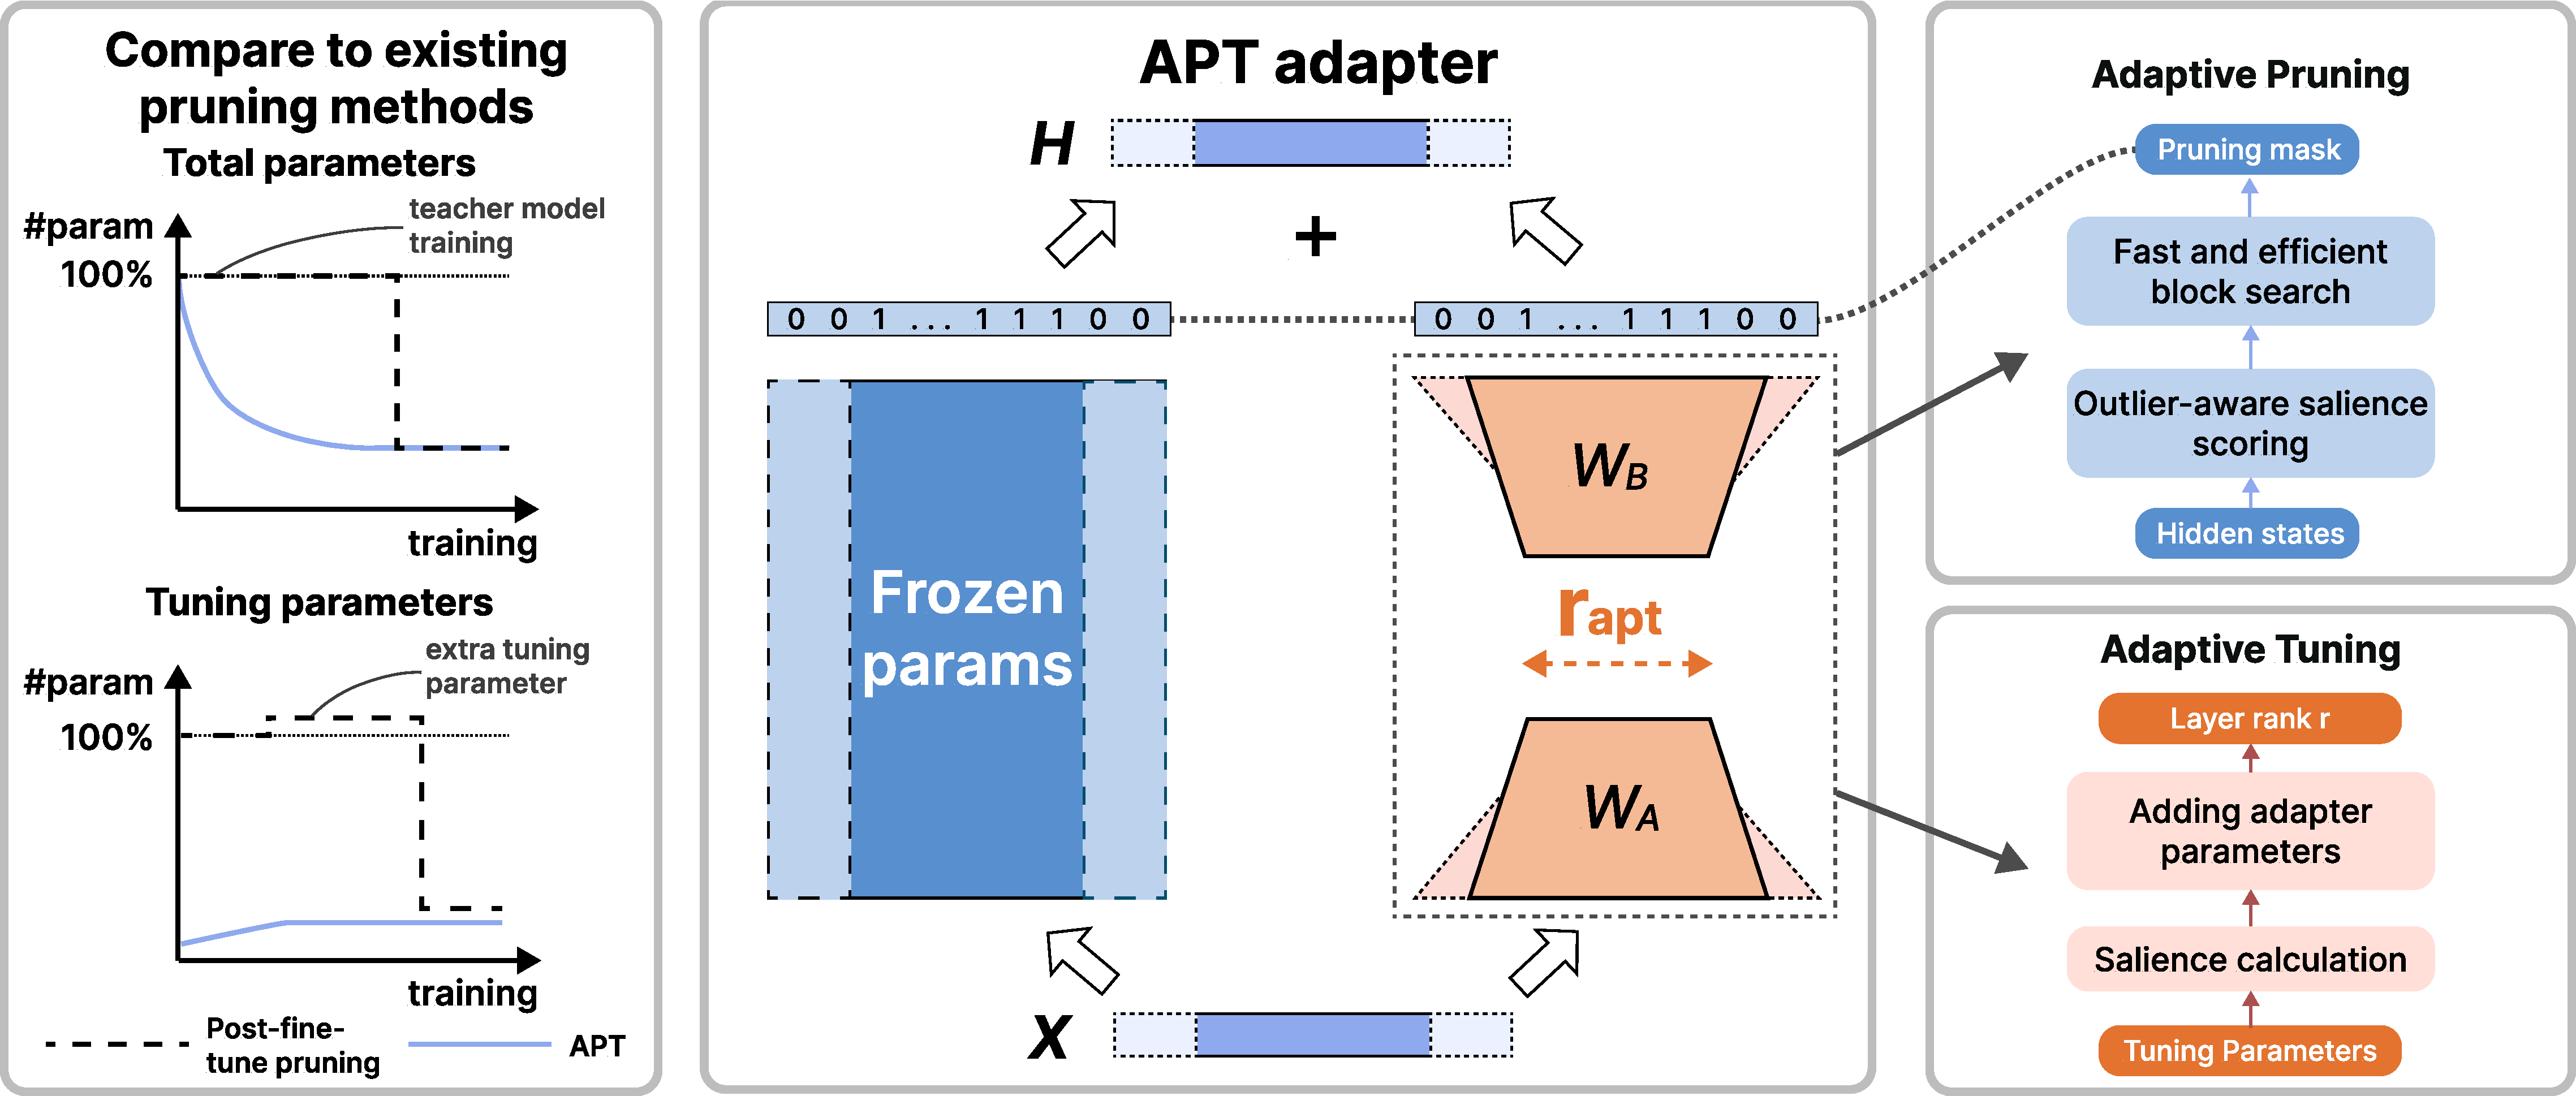
\includegraphics[width=0.95\textwidth]{figures/APT_arch.pdf}
    \caption{{\ourmethod} adaptively identifies pruning and tuning parameters via {\ourarchabbr}s during fine-tuning with little cost. {\ourmethod} gradually prunes {\lmabbr} parameters with binary pruning masks learned from our lightweight outlier-aware salience scoring function for training and inference efficiency. {\ourmethod} also adds tuning parameters in salient layers in {\lmabbr} fine-tuning through increasing dynamic ranks in {\ourarchabbr}s for performance recovery.}
    \label{fig:elastic-adapter}
\vspace{-15pt}
\end{figure*}

We design \textbf{A}daptive \textbf{P}runing and \textbf{T}uning (\textbf{APT}) over {\lmabbr} parameters to allow efficient training and inference while maintaining task performance. 

Summarized in the left of \cref{fig:elastic-adapter}, existing pruning methods often neglect training costs where the number of tuning parameters is more than a parameter-efficient threshold with $\Delta_t \ge \mathcal{C}(\Theta_t, \mathcal{M}_t)$, resulting in long training time and high memory consumption. Instead, to improve training efficiency, we prune {\lmabbr} parameters (increase $\gamma_t$) during early training when $t \ll T$ while keeping $\Delta_t \ll \mathcal{C}(\Theta_t, \mathcal{M}_t)$ to reduce training costs. In addition, we add tuning parameters (increase $\Delta_t$) in early training to effectively mitigate the degradation of {\lmabbr}'s performance due to pruning.

% \subsection{Overview}

% \subsection{{\ourmethod} Overview}
% Some sentences will be moved to the Background section

\noindent \textbf{Overview.} \cref{fig:elastic-adapter} shows the overview of our method that incorporates our new APT adapter for pruning and tuning. Our intuition is that pruning {\lmabbr}s during early fine-tuning will not hurt their task performance while reducing training and inference costs. Meanwhile, unlike existing adapters like LoRA~\cite{hu_lora_2021} that use fixed tuning parameters, APT adapters dynamically add tuning parameters to accelerate {\lmabbr} convergence with superior task performance. We first introduce the architecture of APT adapters in \cref{sec:apt}. We then describe how we prune {\lmabbr} parameters at early fine-tuning with low cost in \cref{sec:apt-prune} and adaptively tune LMs to recover task performance efficiently in \cref{sec:apt-tune}. Additionally, we explain our self-knowledge distillation technique that improves pruned {\lmabbr}'s task performance with limited training expense in \cref{sec:momentum}. 
% during {\lmabbr} fine-tuning, we learn the binary pruning masks via a lightweight outlier-aware salience function with little training cost overhead, and we only add parameters in the top-salient tuning adapters to accelerate convergence with low memory cost.
% \hanna{this is too detailed for an overview; also it has redundancies compared to the opening paragraph, and then lacks motivation why you prune early... Here, just explain the intuition (explained in the intro), then introduce steps according to sub-sections. }
% \hanna{Also, bring  your intuition here -- explained in the intro. }
% \begin{figure}[htbp]
%     \centering
%     \includegraphics[width=\columnwidth]{figures/plot_preliminary_scatter.pdf}
%     \caption{
%     % \hanna{this figure should not be here; maybe it can be moved to the method section or some overview section and only refer to it here}
%     Preliminary study with pruning RoBERTa model on SST-2, where using LoRA with pruning causes large performance degradation while consuming high training time and memory, where {\ourmethod} reaches superior performance and training efficiency.}
%     \label{fig:preliminary}
% \end{figure}

\subsection{{\ourarchabbr}} \label{sec:apt}
We build the {\ourarchabbr} architecture over LoRA, but the key difference is that {\ourarchabbr} supports dynamic {\lmabbr} pruning and tuning. Assuming an {\ourarchabbr} projects the input $X \in \mathbb{R}^{d_i}$ to the output $H_{\text{apt}}(X) \in \mathbb{R}^{d_o}$, we design binary pruning masks ($m_i \in \mathbb{R}^{d_i}$ for input and $m_o \in \mathbb{R}^{d_o}$ for output) and dynamic ranks $r_{\text{apt}}$ in {\ourarchabbr} to control the total and tuning {\lmabbr} parameters during fine-tuning, respectively. Specifically, with tuning parameters $W_A \in \mathbb{R}^{r_{\text{apt}} \times d_i}$ and $W_B \in \mathbb{R}^{d_o \times r_{\text{apt}}}$, {\ourarchabbr} $H_{\text{apt}}$ is denoted as:
\begin{equation} \label{eq:elastic-lora}
        H_{\text{apt}}(X) = m_o \circ (W + s \cdot W_B W_A )X \circ m_i
\end{equation}
where $s$ is the constant scaling factor following LoRA's implementation, and $\circ$ denotes the Hadamard product between the masks and their corresponding matrices. The parameter block is pruned when the multiplying mask is set to 0 and retained when set to 1. In the meantime, during fine-tuning, we dynamically increase $r_{\text{apt}}$ for the weight matrices $W_B$ and $W_A$. Compared to LoRA, APT adapters can be more efficient due to more adaptive pruning and tuning over LM parameters.

In transformer-based {\lmabbr} fine-tuning, we add {\ourarchabbr}s in queries and values of multi-head attention (MHA) layers. We also add {\ourarchabbr} in feed-forward network (FFN) layers when fine-tuning smaller models like RoBERTa and T5 for fast training convergence. In these cases, $m_i$ prunes transformers' hidden dimension and $m_o$ prunes attention heads in MHA and internal neurons in FFN layers. By learning the pruning masks and adjusting the ranks dynamically in the APT adapter, we can achieve the goal defined in \cref{sec:formulation} where the tuning parameter number $\delta(\Theta_t, \mathcal{M}_t, \mathcal{R}_t)$ increases to maintain task performance and the {\lmabbr} parameter size $\mathcal{C}(\Theta_t, \mathcal{M}_t)$ decreases to support more efficient training and inference. Next, we describe the adaptive pruning and tuning procedures in detail.

% Following the notation in \cref{eq: task-formulation}, we can denote {\ourarchabbr} as the layer $\mathcal{E}^k = \{\theta^k, m^k\}$ with the parameter groups $\theta^k = \{W^k, W_B^k,W_A^k, b^k\}$ and masks $M^k=\{m_p^k, m_r^k, m_h^k\}$.


% Based on the {\ourarchabbr} architecture that supports adaptive pruning and tuning, we introduce our Lightweight Parameter Adjustment algorithm to calculate the parameters' salience (weight-gradient production as the importance score) thus identifying and adjusting parameters to be pruned and tuned consuming limited memory. 
% We first introduce how we calculate the approximated parameter salience with outlier awareness, even for those not being tuned, causing limited memory overhead. Afterward, we present our fast knapsack-searching algorithm for transformer pruning. Finally, by combining the parameter pruning and injecting, we show that our Lightweight Parameter Adjustment algorithm can vastly prune a {\lmabbr} with limited resources.

% \begin{equation} \label{eq:sensitivity}
%     \begin{split}
%         % S(W_{i,j}) &= \sum_{(x, y) \in \mathcal{D}} s(W_{i,j}, x, y) \\
%         % &= \sum_{(x, y) \in \mathcal{D}}|\frac{\partial \mathcal{L}(x, y | \Theta)}{\partial W_{i,j}} \cdot W_{i,j}| \\
%         S(W_{:,j}) &= \sum_{(x, y) \in \mathcal{D}}\sum_{i}|\frac{\partial \mathcal{L}(x, y | \Theta)}{\partial W_{i,j}} \cdot W_{i,j}| \\
%         &= \sum_{(x, y) \in \mathcal{D}} (\sum_{i}|\frac{\partial \mathcal{L}(x, y | \Theta)}{\partial X_{j, i}} \cdot X_{j, i}|)
%     \end{split}
% \end{equation}

% \begin{equation} \label{eq:sensitivity}
%     S(m) = |\frac{\partial \mathcal{L}}{\partial m} \cdot m| = \sum_{(X, y) \in \mathcal{D}} |\frac{\partial \mathcal{L}}{\partial H(X)} \cdot H(X)|
% \end{equation}
\subsection{Low-cost Adaptive {\lmabbr} Pruning ($\mathcal{A}_{\text{P}}$)} \label{sec:apt-prune}

% \hanna{this section has some redundancies to previou ssections; it also has too much details that I couldn't follow. Importantly, it is not clear what are novel, what is taken from previous work. }
To benefit the efficiency of LM training and inference, {\ourmethod} adaptively prunes LM parameters since the start of fine-tuning. The problem is finding the parameters to be pruned and discarding them without hurting training stability. Given a task, we compute the outlier-aware salience score of parameter blocks at each early-training step when $t \ll T$. Afterward, we use a fast search algorithm to determine the parameters to be pruned, and then we update their binary pruning masks accordingly. The upper-right of \cref{fig:elastic-adapter} shows this adaptive pruning procedure.

% \hanna{you use the name of outlier-aware salience scoring quite often. Do you introduce this term, or does this exist? instead, you may say we compute a score to obatin saliency of parameters toward an end-task performance? }
% \qq{should describe that pruning happens in two steps, first what metric to decide parameters importance, then do actually pruning, your fast search...}

% \hanna{the following parags can be summarized and made more clear and intuitive; some detailed comments: }
\noindent \textbf{Outlier-aware salience scoring of {\lmabbr} parameters.}
% \qq{for what salience? make it clear, something like ``deciding pruning and tuning parameters" might be better} \bowen{Edited, and I also think the following two sub-subsections shall be compressed later. Or shall they be merged into one?}
When determining the influence of pruning parameters on the {\lmabbr} performance for fine-tuning tasks, the key idea is to compute the outlier-aware salience scores of {\lmabbr} activations to consider both tuning and frozen parameters. 
% \hanna{this sentence about previous work is distracting; maybe move to footnote?}
In detail, salience is defined as the magnitude of parameters' weight-gradient production from previous works~\citep{sanh_movement_2020}, where
\begin{equation} \label{eq:salience}
    S(W_{i, j}) = |{W}_{i,j} \cdot \frac{\partial \mathcal{L}}{\partial {W}_{i,j}}|
\end{equation}

However, since the frozen weights' gradients are unreachable in PEFT settings, we compute the salience as the magnitude of the product of activations and their gradients.
% \hanna{why this product is a representation of a saliency?} \hanna{this next sentence of compression can be moved ot training details.} 
Additionally, we compress the activation and gradients by summing along batches before production to further reduce the training memory consumption. 
% \hanna{don't understand this sentence... have previous work used this? if yes, are you doing exactly the same as previous work, if yes explain it on top}
On the other hand, block outlier parameters play a crucial role in task-specific capabilities, as previous quantization methods suggest~\citep{Dettmers2022LLMint88M,lin2023awq}. Such effects brought by outlier parameters will be averaged if salience is only measured on the block level. To keep more outlier parameters in the pruned {\lmabbr}s, we combine the salience score above and the kurtosis\footnote{Representing the density of the outlier in a distribution, the more the outliers are, the bigger the kurtosis will be.} of the activation together. Therefore, given the supervised finetuning dataset $\mathcal{D}_{t}$, the outlier-aware salience score $\hat{S}$ is defined as:
% \hanna{where did this come from? again ,have other people done it before as well?}
\begin{align}
    % \textrm{Kurt}(X) &= \sum_{(x, y) \in \mathcal{D}} (\sum_i (\frac{X_i - \mu(X)}{\sigma(X)})^4 - 3) \label{eq:kurtosis} \\
    \begin{split}        
        \widetilde{S}_t(W_{:,j}) &= \sum_{(x, y) \in \mathcal{D}_t} \sum_{i} |\frac{\partial \mathcal{L}(x, y | \Theta_t, \mathcal{M}_t)}{\partial H_{j, i}}| \cdot \\
            &\quad \sum_{(x, y) \in \mathcal{D}_t} \sum_{i} | H_{j, i}|
    \end{split} \label{eq:salience-approx} \\
    \hat{S}((W_{:,j}) &= \widetilde{S}(W_{:,j}) + (\textrm{Kurt}(O_{j,:}))^{\frac12} \label{eq:outlier-awared-salience}
\end{align}
where $H$ is the activations in the {\lmabbr}, $\text{Kurt}(\cdot)$ stands for kurtosis, and $O_{:, j} = W_{:, j} \circ X_{j, :}^\intercal$ represents the activation. We leave details of the salience scoring in \cref{appendix:salience-unify}.
% \qq{need to put eq3,4 and 5 together. describe them in one place. First introduce the idea of salience scores, then when describing the details also need to describe why you need them activation instead of parameters, why outlier-aware.}


\noindent \textbf{Efficient search of {\lmabbr} block parameters.}
Given the salience calculated in \cref{eq:outlier-awared-salience}, the next step is to learn the binary pruning masks to increase the {\lmabbr} sparsity above $\gamma_t$. Intuitively, we shall prune the blocks with less salience score, which formulates a latency-saliency knapsack~\citep{NEURIPS2022_5434be94} task.
% To effectively reach the target sparsity, we aim to prune MHA heads, FFN neurons, and the model hidden dimension in transformer-based {\lmabbr}s simultaneously. 
For an {\lmabbr} with $n_L$ transformer layers, where layer $i$ has $n_h^i$ MHA heads and $n_f^i$ FFN neurons, and all transformer layers' hidden dimension sizes are $d_m$, the approximated\footnote{We ignore the model's layer norm and bias terms since their sizes are small, and we do not count tuning parameters since they can be fully merged after training.} number {\lmabbr} parameter is:
\begin{equation} \label{eq:parameter-constraint}
    \mathcal{C}(\Theta_t; \mathcal{M}_t) \approx d_m \sum_{i=1}^{n_L} (4 n_h^i \cdot d_h + 2 n_f^i)
    % &\approx (4 d_h \cdot \sum_h m^h_p + c_f \sum_f m^f_p) \cdot \sum m_h
\end{equation}
where $d_h$ is the dimension per MHA head. To keep the constraint in \cref{eq:problem}, we prune MHA heads, FFN neurons, and the model hidden dimension simultaneously by reducing $n^i_h, n^i_f$, and $d_m$.
% Based on \cref{eq:parameter-constraint}, to reduce the {\lmabbr} parameter $\mathcal{C}(\Theta_t; \mathcal{M}_t)$, we shall decrease $d_m$, $n_h$, and $n_f$ through pruning the hidden dimension, MHA heads, and FFN neurons. 
% \hanna{it seems yepeat the same thing over and over with different wording. First, explain the intuition, then explain the exact thing that you did; the next few sentences are much more clear and probably the most important things in this section, bring them on top.}
Hence, we first sort the blocks by their salience divided by the parameter number. As the parameter size monotonically increases with block quantity, we use binary search to identify the top salient blocks to be retained given the sparsity constraint $\gamma_t$. 
% \hanna{the next few sentences can also be moved into training datails.
We leave the implementation details in \cref{appendix:binary-search} for simplicity.

\subsection{Adaptive and Efficient LM Tuning ($\mathcal{A}_{\text{T}}$)} \label{sec:apt-tune}
% Low-cost lightweight, or what
% Intuitive overall concept -> detail -> equations
% \qq{need a few sentences to describe how tuning works}
As using PEFT methods to fine-tune pruned {\lmabbr}s causes notable performance decrease (illustrated in \cref{tab:small-model-results} and \cref{tab:ablate-paramalloc}), we aim to dynamically add tuning parameters in {\lmabbr} fine-tuning to improve the model's end-task performance. However, since more tuning parameters will consume extra training time and memory, we want to add parameters in a controlled way, where new parameters are only added to task-sensitive {\ourmethod} adapters. As a result, we can recover pruned {\lmabbr}s' performance with reasonable training costs.
% \todo{why adding parameters: 1. pruned LM performance downgrade; 2. less parameter -> less performance but faster and less memory; 3. efficiency is reasonable, but recovering performance}
% Now we present our procedure of adding tuning parameters in salient {\lmabbr} layers for effective {\lmabbr} performance recovery after pruning as depicted in the lower-right section of \cref{fig:elastic-adapter}. To balance training efficiency and performance, we aim to add parameters in a subset of tuning adapter layers selected based on salience \qq{clarify}. \todo{connect to 4.1 above (APT adapters)}
In detail, we first calculate the salience of each {\ourmethod} adapter to determine their importance. Next, we select the top-half {\ourmethod} adapters after sorting them with salience and add their parameters by increasing their $r_{\text{apt}}$.

\noindent \textbf{Salience scoring of {\ourarchabbr}.}
% \hanna{doesn't section 4.3 explain how you compute LM parameter saliency? just refer to it. you can say Given saliency scores of LM parameters (4.2), we define the layer saliency in APT adapter? ... }
Since gradients of tuning parameters information are available when determining the layer salience, we can first calculate each tuning parameter's salience with \cref{eq:salience}. Then, we define the salience of an APT adapter as the summation of the parameter salience scores in $W_B$, denoted as $\mathcal{I}(H_{\text{apt}}) = \sum_{i, j}S({W_B}_{i, j})$, to represent each tuning {\ourarchabbr}'s importance\footnote{The salience scores calculated using $W_B$ and $W_A$ are equal, so using either of them will get the same result.}. Given the calculated $\mathcal{I}(H_{\text{apt}})$ for each {\ourarchabbr}, we can then decide where to add new tuning parameters to efficiently improve the pruned {\lmabbr}'s task accuracy.

\noindent \textbf{Dynamically adding APT adapter parameters to recover task performance.} 
With the importance of {\ourarchabbr}s $\mathcal{I}(H_{\text{apt}})$ calculated, the next step of adaptive tuning is to add tuning parameters by increasing the salient tuning layers' ranks $r_{\text{apt}} \in \mathcal{R}_t$ following budget $\Delta_t$. Therefore, firstly, we sort all tuning layers according to their importance score $\mathcal{I}(H_{\text{apt}})$ and linearly increase the ranks of the top-half salient ones. More specifically, when increasing the tuning parameter from $\Delta_t$ to $\Delta_{t'}$, the salient layer's rank is changed from $r_{\text{apt}}$ to $r_{\text{apt}}' = \lfloor r_{\text{apt}} \cdot \frac{\Delta_{t'}}{\Delta_t} \rfloor$ where $\lfloor \cdot \rfloor$ denotes the floor operation. For training stability, when adding parameters and converting $W_B \in \mathbb{R}^{d_o \times r_{\text{apt}}}, W_A \in \mathbb{R}^{r_{\text{apt}} \times d_i}$ to $W_B' \in \mathbb{R}^{d_o \times r_{\text{apt}}'}, W_A' \in \mathbb{R}^{r_{\text{apt}}' \times d_i}$, we concatenate random Gaussian initialized parameters $\mathcal{N}(0, \sigma^2)$ in $W_A$ and zeros in $W_B$ same as the LoRA initialization, so the layer's output remains unchanged before and after new parameters added.

% Existing fine-pruning methods cost longer training time because of joint optimization of parameters and masks. To speed up training, we propose our fast-searching method to prune a transformer model's blocks (MHA heads, FFN neurons, and hidden dimensions) purely based on salience scores from \cref{eq:outlier-awared-salience} without extra controlling modules. 



% \qq{you need to provide context why you need to allocate parameters for tuning, is it because the performance drop, or for efficiency tradeoffs, etc.}
% To tackle the performance downgrade challenge, we linearly increase the top-half salient tuning layers' LoRA weights in training. To control memory usage, we also discard stably unimportant parameters at the early stage. As shown in \cref{tab:ablate-paramalloc}, we can see that adjusting the layer's parameter size based on salience always yields better results.

% Furthermore, with the scoring function defined in \cref{eq:salience-approx}, we can conduct pruning before tuning to further reduce the memory consumption as shown in \cref{tab:llama-7b-results}. For the pruning during tuning, 
% Overall, our Lightweight Parameter Adjustment algorithm is summarized as \cref{alg:epa} while the schedule is as depicted in \cref{fig:schedule}.



\subsection{Efficient Self-Knowledge Distillation} \label{sec:momentum}
% \qq{This section can be compressed, too many details, you can start with why the Self-Momentum Distillation is needed, due to accuracy drop? and then how you can improve accuracy w/o extra overhead due to distillation (because naive distillation causes memory overhead, making training inefficient.) Summarize the key techniques you used, briefly describe the key ideas and how they improve performance without overhead} 
As shown in \cref{tab:ablate-paramalloc}, training pruned {\lmabbr} without knowledge distillation causes significant end-task performance drops. Therefore, we use knowledge distillation in {\ourmethod} to recover the pruned {\lmabbr}'s performance. Still, existing strategies require a fully trained teacher model being put into the GPU with the student during distillation, causing high training time and memory. To avoid extra training costs, we keep duplicating the tuning student layers as teachers during fine-tuning to reduce total training time. Meanwhile, frozen parameters are shared between the student and teacher model during training to reduce memory consumption. We edit the distillation objective in CoFi~\citep{xia_structured_2022} as
% Furthermore, after the student model's pruning masks are settled and fixed, we select student layer weights using masks $m_p$ and $m_h$ from the shared weights instead of conducting multiplication in high-sparsity pruning settings for further training memory reduction. 
\begin{equation}
    \begin{split}
        % \mathcal{L} &= \mu (\lambda \mathcal{L}_{pred} + (1 - \lambda) \mathcal{L}_{layer}) + (1 - \mu) \mathcal{L}_{ft} \\
        \mathcal{L} &= \mu \mathcal{L}_{distill} + (1 - \mu) \mathcal{L}_{ft} \\
        \mathcal{L}_{layer} &= \sum_{i=1}^\mathcal{T} \textrm{MSE}(\text{Tr}(H_s^{\phi(i)}), H_t^i)
    \end{split}
\end{equation}
where $\mu$ is a moving term linearly scales from 0 to 1 during distillation to encourage the pre-pruned model vastly fit to the training data, $\mathcal{L}_{distill}$ is the distillation objective from CoFi, and $\mathcal{L}_{ft}$ is the supervised fine-tuning objective. $\mathcal{T}$ is block-wise randomly sampled teacher layers following~\citep{haidar2022rail}, $\phi(\cdot)$ is the teacher-student layer-mapping function that matches the teacher layer to its closest, non-pruned student layer. $\text{Tr}$ denotes the tunable LoRA layer for layer transformation, initialized as an identical matrix $\mathcal{I}$. More implementation details of our self-distillation technique is introduced in \cref{appendix:hyper-param}.

% \noindent \textbf{Dynamic layer mapping for better pruning adaptivity.} As for selecting the teacher layers $\mathcal{T}$ during each training step, we randomly sample $n$ layers from the teacher model since existing research found that this strategy yields better distillation results. However, we find that dynamic teachers combined with the dynamic student selection method from CoFi would result in layer-shifting (only bottom student layers are selected, even though the teacher comes from the top), especially in larger encoder-decoder models like T5. Besides, we find that the advantage of CoFi's distillation mainly comes from the layer mapping when the student layer is entirely pruned. Therefore, for the layer mapping function $\phi(\cdot)$, we will do a static mapping if the corresponding layer is not being pruned in the student model, or otherwise, we would dynamically map it to the most similar neighbor layer in the student model:
% \begin{equation}
% \begin{split}
%   \phi(i) &= \displaystyle\argmin_{j \in n(i)} \text{MSE}(W_{tr} H_s^j, H_t^i)
% \end{split}
% \end{equation}
% where $n(i)$ denotes the preserved neighbor layers of the pruned layer, either on its top or bottom. Empirically, this strategy will always find the most effortless teacher layer for student layers to be learned from without raising any layer-shifting problem. 
\section{Experiments}

% % Please add the following required packages to your document preamble:
% \usepackage{booktabs}
% \begin{wraptable}{l}{0.6\textwidth}
\begin{table*}[htbp]
\begin{tabular}{@{}l|lrr|llll@{}}
\toprule
Method                    & MNLI                           & SST2                           & SQuAD v2                       & Train. Speed & Train. Mem. & Inf. Speed & Inf. Mem. \\ \midrule
FT                        & 87.6                           & 94.8                           & 82.9                           & 100.0\%      & 100.0\%     & 100.0\%    & 100.0\%   \\
LoRA                      & 87.5                           & 95.1                           & 83.0                           & 4.7\%        & 60.5\%      & 100.0\%    & 100.0\%   \\ \midrule
LoRA + Prune              & 84.0                           & 93.0                           & 79.2                           & 2.0\%        & 60.5\%      & 262.9\%    & 75.1\%    \\
LoRA + Distill            & 84.2                           & 91.9                           & -                              & 1.5\%        & 141.4\%     & 253.7\%    & 82.3\%    \\ \midrule
\ourmethod & \textbf{86.4} & \textbf{94.5} & \textbf{81.8} & 16.9\%       & 70.1\%      & 241.9\%      & 78.1\%    \\ \bottomrule
\end{tabular}
\caption{RoBERTa pruning with {\ourmethod} compared to baselines under 60\% sparsity. We measure the training and inference efficiency with {\lmabbr}s pruned on the SST2 task. Training speed is measured via 97\% accuracy TTA.}
\label{tab:main-result}
% \vspace{-15pt}
\end{table*}

% % Please add the following required packages to your document preamble:
% \usepackage{booktabs}
\begin{table*}[htbp]
\centering
\begin{tabular}{@{}l|rlr|llll@{}}
\toprule
Method                        & MNLI                           & SST2                           & CNN/DM                                                                                       & Train. Speed & Train. Mem. & Inf. Speed & Inf. Mem. \\ \midrule
FT                            & 87.1                           & 95.2                           & 42.1/20.3/39.4                                                                               & 100.0\%      & 100.0\%     & 100.0\%    & 100.0\%   \\
LoRA                          & 87.0                           & 95.0                           & 38.7/17.2/36.0                                                                               & 39.1\%       & 62.0\%      & 100.0\%    & 100.0\%   \\ \midrule
LoRA + Prune                  & 80.9                           & 92.3                           & 36.7/15.7/33.9                                                                               & 2.5\%        & 62.0\%      & 212.5\%    & 73.4\%    \\ \midrule
{\ourmethod} & \textbf{87.0} & \textbf{95.0} & \textbf{38.6}/\textbf{17.0}/\textbf{35.8} & 20.6\%       & 73.9\%      & 134.1\%    & 81.5\%    \\ \bottomrule
\end{tabular}
\caption{T5 model pruning with {\ourmethod} compared to existing baselines under 60\% sparsity. We measure the training and inference efficiency with {\lmabbr}s pruned on the SST2 task. Training speed is measured via 97\% accuracy TTA.}
\label{tab:t5-main-results}
\vspace{-15pt}
\end{table*}
% Please add the following required packages to your document preamble:
% \usepackage{booktabs}
% \usepackage{multirow}
\begin{table*}[t!]
\resizebox{1.0\linewidth}{!}{
\begin{tabular}{@{}ll|rrrr|rrrr@{}}
\toprule
Model                                           & Method         & MNLI          & SST2          & SQuAD v2      & CNN/DM                  & Train Time($\Downarrow$) & Train Mem($\Downarrow$) & Inf Time($\Downarrow$) & Inf Mem($\Downarrow$) \\ \midrule
\multirow{5}{*}{$\text{RoBERTa}_{\text{base}}$} & FT             & 87.6          & 94.8          & 82.9          & -                       & 100.0\%      & 100.0\%     & 100.0\%    & 100.0\%   \\
                                                & LoRA           & 87.5          & 95.1          & 83.0          & -                       & 2137.0\%        & 60.5\%      & 100.0\%    & 100.0\%   \\ \cmidrule(l){2-10} 
                                                & LoRA+Prune   & 84.0          & 93.0          & 79.2          & -                       & 5128.3\%        & \textbf{60.5\%}      & \textbf{38.0\%}    & \textbf{75.1\%}    \\
                                                & Prune+Distill   & \textbf{87.3}          & \textbf{94.5}          &   -        & -                       & 1495.3\%        & 168.5\%      & 38.6\%    & 79.2\%    \\
                                                & LoRA+Prune+Distill & 84.2          & 91.9          & -             & -                       & 6534.6\%        & 141.4\%     & 39.4\%    & 82.3\%    \\  \cmidrule(l){2-10} 
                                                & \ourmethod     & 86.4 & \textbf{94.5} & \textbf{81.8} & -                       & \textbf{592.1\%}       & 70.1\%      & 41.3\%    & 78.1\%    \\ \midrule
\multirow{4}{*}{$\text{T5}_{\text{base}}$}      & FT             & 87.1          & 95.2          & -             & 42.1/20.3/39.4          & 100.0\%      & 100.0\%     & 100.0\%    & 100.0\%   \\
                                                & LoRA           & 87.0          & 95.0          & -             & 38.7/17.2/36.0          & 255.5\%       & 62.0\%      & 100.0\%    & 100.0\%   \\ \cmidrule(l){2-10} 
                                                & LoRA+Prune   & 80.9          & 92.3          & -             & 36.7/15.7/33.9          & 4523.5\%        & \textbf{62.0\%}      & \textbf{47.1\%}    & \textbf{73.4\%}    \\ \cmidrule(l){2-10} 
                                                & \ourmethod     & \textbf{87.0} & \textbf{95.0} & -             & \textbf{38.6/17.0/35.8} & \textbf{484.7\%}       & 73.9\%      & 74.6\%    & 81.5\%    \\ \bottomrule
\end{tabular}
}
\caption{RoBERTa and T5 pruning with {\ourmethod} compared to baselines under 60\% sparsity. We measure the training and inference efficiency with {\lmabbr}s pruned on the SST2 task. Training speed is measured via 97\% accuracy TTA. All efficiency metrics are normalized to FT. $\Downarrow$ denotes smaller is better. The best-pruned results are \textbf{bold}. Raw efficiency results are reported in \cref{tab:raw-efficiency}.}
\label{tab:small-model-results}
\vspace{-5pt}
\end{table*}

% Please add the following required packages to your document preamble:
% \usepackage{booktabs}
% \usepackage{multirow}
\begin{table*}[htbp]
\centering
\resizebox{1.0\linewidth}{!}{
\begin{tabular}{@{}l|rrrrr|rrrr@{}}
\toprule
Method       & ARC                            & HellaSwag                      & MMLU                           & TruthfulQA                     & Avg.                           & Train Time($\Downarrow$) & Train Mem ($\Downarrow$) & Inf Time($\Downarrow$) & Inf Mem($\Downarrow$) \\ \midrule
LLaMA 2 7B   & 53.1                           & 77.7                           & 43.8                           & 39.0                           & 53.4                           & -            & -           & -          & -         \\ 
LoRA         & 55.6                           & 79.3                           & 46.9                           & 49.9                           & 57.9                           & 100.0\%      & 100.0\%     & 100.0\%    & 100.0\%   \\ \midrule
LoRA+Prune & \textbf{46.8} & 65.2                           & 23.9                           & 46.2                           & 45.5                           & 180.9\%       & 100.0\%     & 115.5\%    & 68.9\%    \\
LLMPruner    & 39.2                           & 67.0                           & 24.9                           & 40.6                           & 42.9                           & \textbf{86.9\%}      & 253.6\%     & \textbf{114.8\%}    & 74.2\%    \\ \midrule
APT          & 45.4                           & \textbf{71.1} & \textbf{36.9} & \textbf{46.6} & \textbf{50.0} & 106.0\%       & \textbf{75.8\%}      & 117.0\%    & \textbf{67.2\%}    \\ \bottomrule
\end{tabular}
}
\caption{
% \hanna{this table has a different set of baelines, explain why you are using a diferent baseline here. }
    LLaMA 2 7B 30\% sparsity pruning results with GPT4-generated Alpaca dataset, evaluated on the Open LLM leaderboard few-shot tasks. Training speed is measured via training time per step. We do not compare to distillation baselines because the training cost of distillation is too large, and we also compare {\ourmethod} to LLMPruner since it is dedicated to large {\lmabbr} pruning. All efficiency metrics are normalized to LoRA. $\Downarrow$ denotes smaller is better. The best-pruned results are \textbf{bold}. Raw efficiency results are reported in \cref{tab:raw-llama-efficiency}.}
\label{tab:llama-7b-results}
\vspace{-15pt}
\end{table*}

To evaluate the training and inference efficiency gains of {\ourmethod}, we compare it with the combined use of PEFT with pruning and distillation baselines. We first describe the natural language understanding and generation tasks targeting different {\lmabbr} backbones, then the setup of baselines and {\ourmethod}. We then report task performance, speed, and memory usage for training and inference costs. 
% \qq{add a few sentences for the evaluation overview.}

\subsection{Tasks}
% \hanna{it seems that you also apply APT to llama based models, right? in that case, start with this: We add APT to the following language models, bert, roberta, T5 and llama; for bert and t5, we evaluate on ... For llama, we evaluate on ... , following... }

We apply {\ourmethod} to BERT~\citep{devlin-etal-2019-bert}, RoBERTa~\citep{liu2019roberta},  T5\citep{raffel2020exploring}\footnote{For fair comparisons, we use the t5-lm-adapt model, which is only pre-trained on the C4 corpus to make sure the initial {\lmabbr} does not observe downstream tasks in pre-training.}, and LLaMA~\citep{touvron2023llama}. 
For BERT, RoBERTa, and T5 models, we train and evaluate on SST2 and MNLI datasets from the GLUE benchmark~\citep{wang2018glue} and report the dev set accuracy. We also train and evaluate $\text{RoBERTa}_{\text{base}}$ on SQuAD v2.0~\citep{rajpurkar-etal-2018-know} and report the dev set F1 score. For T5 models, we also fine-tune them on CNN/DM~\citep{Nallapati2016AbstractiveTS} and report the ROUGE 1/2/L scores. Meanwhile, We use the GPT-4 generated Alpaca dataset~\citep{alpaca} to fine-tune large LLaMA models and evaluate them with the lm-eval-harness package~\citep{eval-harness} on four tasks from the Open LLM Leaderboard, namely 25-shot ARC~\citep{clark2018think}, 10-shot HellaSwag~\citep{zellers-etal-2019-hellaswag}, 5-shot MMLU~\citep{hendrycks2021measuring}, and zero-shot TruthfulQA~\citep{lin-etal-2022-truthfulqa}.
% and AlpacaEval~\citep{alpaca_eval} to test the model's generalization and instruction-following capabilities.

\subsection{Baselines}
% \hanna{provide a high level overview of what type of baselines you are slecting here? only PEFT methods? only pruning methods? then basic approaches for prune + PEFT, then sota approaches for prune + PEFT? }
% \qq{the first key baseline is Adapter+Pruning (in our case LoRA+Prune), we compare both the training and inference efficiency. Then you can describe other baselines to compare either training or inference efficiency. Also remember the two goals for our work, we make smaller models faster during training with more memory? and we make larger models train less memory while inference is still faster etc. Describe the baselines for these two scenarios. }

% Since {\ourmethod} optimizes training and inference efficiency together with task performance, we compare it to baselines that jointly use PEFT and pruning. 
% \bowen{I get it. Probably only mentioning the mixed-use baselines are enough, instead of pointing out FT, LoRA individually. I'll revise it later.}

% \noindent \textbf{Fine-tuning (FT)}. We compare {\ourmethod} to full fine-tuning without pruning on million-parameter scaled language models, where all parameters except for the embedding weights (in-line with existing structured pruning settings) are being tuned simultaneously. We do not compare our method to full fine-tuning with billion-level {\lmabbr}s, since the memory consumption would be too large to fit in single-card GPU training settings, where most parameter-efficient methods could.

% \noindent \textbf{LoRA}~\citep{hu_lora_2021} tunes language models with low-rank adaptation. Similar to existing usages of LoRA, we only tune the query and value layers in all MHA layers, including self-attention and cross-attention, with the inner rank set as 8 and the scaling factor set as 2. 
We validate the efficiency benefits of {\ourmethod} for both training and inference by comparing with PEFT, pruning, and distillation methods, along with their combinations. 

\noindent \textbf{LoRA+Prune}: a post-training pruning method over on LoRA-tuned {\lmabbr}s. We use Mask Tuning~\citep{kwon_fast_2022}, a state-of-the-art post-training structured pruning method based on fisher information. Due to that post-training pruning performs poorly on high-sparsity settings, we retrain the pruned {\lmabbr} after pruning to recover its performance.
% We apply MT to LoRA-tuned models and also add two baselines $\text{MT}_{\text{+train}}$ and $\text{MT}_{\text{+distill}}$ denoting conducting retraining or distilling with LoRA after MT.
% \qq{this also has pruning? then we should name it LoRA+Prune+distillation}

% \todo{CoFi without LoRA, fully fine-tuning on RoBERTa -> Pruning + Distillation}

\noindent \textbf{Prune+Distill}: knowledge distillation has been proved to be a key technique in recovering pruned {\lmabbr}s' task accuracy. In particular, we use the state-of-the-art pruning plus distillation method called CoFi~\citep{xia_structured_2022} which uses $L_0$ regularization for pruning plus dynamic layer-wise distillation objectives. We only compare {\ourmethod} to CoFi with RoBERTa models since the training memory usage of CoFi is too high for larger {\lmabbr}s.

\noindent \textbf{LoRA+Prune+Distill}: to reduce the training memory consumption in pruning and distillation, a simple baseline is to conduct CoFi pruning and distillation but with LoRA parameters tuned only. More specifically, only the $L_0$ module and LoRA parameters are tunable under this setting.  

\noindent \textbf{LLMPruner}~\citep{ma2023llm}: LLMPruner is the state-of-the-art task-agnostic pruning method on LLaMA that prunes its blocks or channels based on salience metrics while using LoRA for fast performance recovery. We compare {\ourmethod} to LLMPruner with fine-tuning on the same GPT-4 generated Alpaca data for fair comparisons.

We also compare {\ourmethod} to PST~\citep{ijcai2022p586} and LRP~\citep{zhang2023pruning}, which are the state-of-the-art parameter-efficient unstructured and structured pruning methods on $\text{BERT}$ model. We leave these results in \cref{sec:appendix-additional-exp}.

% \noindent \textbf{LLM-pruner} \bowen{also comparing to it on LLaMA 2 if have time}


\subsection{Evaluation Metrics}
% \hanna{start this paragraph with a title evaluation metrics} 
% \hanna{all these are scattered. You need to organize them better. Start with Training Efficiency metrics: we report ... then, Inference efficiency metrics: ... } 
We evaluate {\ourmethod} and baselines on training and inference efficiency, measured in runtime memory and time consumption as follows:

\noindent\textbf{Training Efficiency Metrics}: we report relative training peak memory (Train. Mem.) and relative training speed measured by time to accuracy (TTA\footnote{For instance, 97\% TTA denotes the time spent reaching 97\% of the fully fine-tuned model's performance})~\citep{10.1145/3352020.3352024} compared to full finetuning. For fair comparisons, we consider the training time of the teacher model plus the student for methods using knowledge distillation.

\noindent\textbf{Inference Efficiency Metrics}: we report the inference peak memory (Inf. Mem.) and the relative speedup (Inf. Speed) based on throughput (data processed per second) for inference efficiency. 

Both training and evaluation are conducted on a single A100 GPU. The inference test batch size is 128 for small models while 32 and 4 for LLaMA 7B and 13B models, respectively. We demonstrate detailed training and evaluation setups/implementations in \cref{appendix:hyper-param}.

\subsection{Main Results} \label{sec:main-result}
% \bowen{training AND inference efficiency -> detail, memory or time, how much. what experiments are conducted, detailed results and provide contexts}
% \qq{you want to highlight that our method achieves both the training and inference efficiency goal, show the key results over baselines. LoRA+Prune is an evidential example. First describe the results. Then describe the results detail.}

% \hanna{refer to table 2 here; table 2 shows the main results... Here, you can mention, APT generally doesn't hurt accuracy in most settings, while improving training ... [a precise term here] and refer to the details below.  }

% \hanna{I would categorize the results better. what are the main points you want to highlight. 1. compare APT with FT and LORA. APT improves training speed compared to FT and decreases memory by ... with ... cost at accuracy in both small and large lms. 2. compare APT with other peft and prune methods. 3. comapre apt with the distill models. }
% \todo{speedup compared to which baseline, be specific}
\noindent \textbf{Overview} We demonstrate the end-task performance of {\ourmethod} comparing to fine-tuning (FT), LoRA-tuning (LoRA), and pruning baselines in \cref{tab:small-model-results} and \cref{tab:llama-7b-results}. Overall, up to 99\% of fine-tuned {\lmabbr}'s task accuracy is maintained when pruning RoBERTa and T5 models leaving 40\% parameters, with only about 70\% training memory consumption than fine-tuning. When pruning LLaMA2-7B models with 70\% parameters remaining, {\ourmethod} recovers 86.4\% task performance on average, together with only 75.8\% training memory usage than LoRA-tuning. Furthermore, {\ourmethod} also significantly reduces end-task performance and training costs compared to the pruning and distillation baselines. The detailed comparisons are shown as follows.

\noindent \textbf{{\ourmethod} speeds up RoBERTa and T5 training 8$\times$ and reduces training memory costs to 30\% in LLaMA pruning compared to LoRA+Prune baseline.} 
% \todo{Highlight the advantages of {\ourmethod} -> efficiency. performance better in what conditions? Extracting main messages.}
% \qq{put this section to be the first main results}
% \qq{this is not accurate, describe clearly what efficiency for training or inference, e.g., our method speeds up small model training, xxx}
% with only 15.9\% and 19.2\% extra memory costs
% \todo{add detailed values, e.g., 2-8 times and xx\% memory usage}
Shown in \cref{tab:small-model-results}, when pruning RoBERTa models to 60\% sparsity, {\ourmethod} converges $8.4\times$ faster than the LoRA+Prune baseline with consuming similar GPU memory. {\ourmethod} also prunes T5 models 8.2$\times$ faster than the LoRA+Prune baseline. The reason is that {\ourmethod} adaptively prunes task-irrelevant parameters during training, reducing memory and per-step training time. Adding parameters in salient tuning layers also accelerates {\lmabbr} convergence. 
Also, {\ourmethod} costs less than 24GB of memory when pruning 30\% parameters in LLaMA2-7B models before tuning, which can be easily adapted to the consumer-level GPUs. In contrast, LLM-Pruner costs about 80GB memory when pruning the LLaMA 7B model\footnote{\url{https://github.com/horseee/LLM-Pruner/issues/4}}.

\noindent \textbf{{\ourmethod} achieves 2.5\%-9.9\% higher task performance than the LoRA+Prune baseline with the same pruning sparsities.} 
% \todo{performance superior to which baseline (LoRA+Prune)}
% \todo{how much performance improved, improves xx\% higher}
Presented in \cref{tab:small-model-results} and \cref{tab:llama-7b-results}
, when RoBERTa, T5, and LLaMA models, regardless of size, {\ourmethod} consistently reach higher task performance than the LoRA+Prune. 
% In detail, when pruning 60\% parameters, {\ourmethod} effectively recovers 99.4\% LoRA-tuned {\lmabbr} performance on average, while the LoRA+Prune baseline can only maintain 95.6\% performance. 
With similar inference speedup and memory when pruning RoBERTa models, {\ourmethod} reaches 2.5\% more end-task performance on average.
% Moreover, {\ourmethod} performs the same with the LoRA baseline on T5 classification tasks (SST2 and MNLI) without any performance loss. 
When pruning T5 models under the 60\% sparsity, the task performance achieved by {\ourmethod} is 5.1\% better than the LoRA+Prune baseline. However, the inference efficiency reached by {\ourmethod} (1.3$\times$ speedup and 81.5\% memory cost) is worse than the LoRA+Prune baseline (2.1$\times$ speedup and 73.4\% memory cost). This is because {\ourmethod} can adaptively prune more decoder parameters, which are also computationally cheaper than encoder parameters (due to shorter output sequence length) but relatively useless for classification tasks. 
% In the meantime, {\ourmethod} maintains 98.9\% LoRA tuning performance in generation tasks like CNN/DM, showing the capabilities of being used under generative settings.
% Furthermore, it shall be noticed that static LoRA tuning on the T5-base model for the CNN/DM task causes performance degradation. The reason is that for generative tasks, the ranks for LoRA tuning shall be set larger empirically. Therefore, with our {\ourarchabbr} architecture that expands its parameters during training, it is viable to tune generative models with lower peak memory consumption.
For LLaMA2-7B model pruning with 70\% sparsity, {\ourmethod} outperforms LLMPruner with 16.5\% and the LoRA+Prune baseline with 9.9\%, where the inference efficiency improvements of {\ourmethod} is slightly better than both LoRA+Prune and LLMPruner baselines. 
% For TruthfulQA, which shows the most gain through fine-tuning (39.0 to 49.9), both LoRA+Prune (46.2) and LLMPruner (40.6) can recover models' ability. However, these baselines fail to perform as well on other tasks such as MMLU (23.9 for MT-retrained and 24.9 for LLMPruner, worse than random guessing). This performance trajectory shows that the prune-then-retrain paradigm could harm large {\lmabbr}'s generalization capabilities when sub-optimal parameter pruning results are reached.

% \hanna{I don't think the following statement is accurate. You first need to explain Figure 3 and then explain the finding. I don't fully understand this result. Don't make innacurate stamenets boldface. }
% \todo{move this to forward and merge}
% \noindent \textbf{{\ourmethod} prunes {\lmabbr}s with 6\% to 60\% more inference speedup and reduces inference 7\%-25\% more memory with similar task performance.} 
% \todo{how much inference efficiency gained}

% \todo{Add comparison to Prune+Distill baseline, better training efficiency}
\noindent \textbf{{\ourmethod} reaches on-par performance with the Prune+Distill baseline given the same pruning sparsity but trains 2.5$\times$ faster and costs only 41.6\% memory.}
Compared to the Prune+Distill baseline, {\ourmethod} results in comparable task accuracy (0.9 point drop in MNLI and same in SST2). At the same time, with similar inference efficiency achieved, {\ourmethod} costs only 41.6\% training memory and converges 2.5$\times$ than the Prune+Distill baseline. This is because of the self-distillation technique in {\ourmethod} where no separated teacher model is required in pruning {\lmabbr}s. Moreover, {\ourmethod} achieves better task performance than the LoRA+Prune+Distill baseline as well, with less training time and memory consumption. These results demonstrate that {\ourmethod} successfully tackles the problem where simply combining PEFT and pruning hurts pruned {\lmabbr}'s task accuracy and training efficiency.

% \begin{figure}[htbp]
%     \centering
%     \includegraphics[width=\columnwidth]{figures/llama2_7b_tradeoff.pdf}
%     \caption{The average performance of LLaMA 2 7B model pruning against relative training and inference memory usage along with inference speedup. The numbers beside each point denote the pruning sparsity.}
%     \label{fig:llama-tradeoff}
%     \vspace{-10pt}
% \end{figure}

% \qq{since here you only discuss inference efficiency, I assume the previous section is about training efficiency, you might want to adjust the title}
% Regarding the inference efficiency, {\ourmethod} reaches similar time and memory costs compared to the LoRA+Prune baseline when pruning RoBERTa models. However, when pruning T5 models, since {\ourmethod} prunes more parameters in the decoder that causes less computation when performing the SST2 classification task, {\ourmethod} results in relatively worse inference efficiency when the similar amount of parameters are pruned. On the other hand, {\ourmethod} achieves superior inference efficiency in throughput and memory when pruning LLaMA models than existing baselines. Overall, {\ourmethod} improves the model inference efficiency similar to baselines for encoder- and decoder-only {\lmabbr}s, but for encoder-decoder {\lmabbr}s, the inference efficiency gain is dependent on the property of fine-tuning tasks (classification or generation).

% % Please add the following required packages to your document preamble:
% \usepackage{booktabs}
\begin{table}[]
\begin{tabular}{@{}lr|rrrr@{}}
\toprule
Method                         & Density & SST2 & CNN/DM &  T. M. & Inf. Speedup \\ \midrule
FT                           & 100\%   & 97.4 &  42.72/21.02/39.94  &            &              \\
LoRA                           & 100\%   & 97.5 &        &            &              \\ \midrule
LoRA + $\text{MT}_{\text{train}}$            & 8\%    &   83.1  &         &       &              \\
LoRA + $\text{MT}_{\text{distill}}$            & 8\%    & 90.9  &           &       &              \\
{\ourmethod}                  & 8\%    &  92.0  &        &          &              \\ \bottomrule
\end{tabular}
\caption{T5-XL results}
\label{tab:t5-3b-results}
\end{table}
% \begin{figure}[t!]
%     \begin{minipage}{0.48\textwidth}
%         \begin{figure}[H]
%             \centering
%             \includegraphics[width=\textwidth]{figures/plot_training_tradeoff_scatter.pdf}
%             \caption{Caption}
%             \label{fig:enter-label}
%         \end{figure}
%     \end{minipage}
%     \hfill
%     \begin{minipage}{0.48\textwidth}
%         \begin{figure}[H]
%             \centering
%             \includegraphics[width=\textwidth]{figures/plot_inference_tradeoff_scatter.pdf}
%             \caption{Caption}
%             \label{fig:enter-label}
%         \end{figure}
%     \end{minipage}
% \end{figure}

% % Please add the following required packages to your document preamble:
% \usepackage{booktabs}
\begin{table*}[htbp]
\centering
\begin{tabular}{@{}lr|rrrrrr@{}}
\toprule
Method                         & Density & SST2 & 97\% TTA     & 99\% TTA     & T. M. & Inf. $\nearrow$ & Inf. Mem. \\ \midrule
FT                             & 100\%   & 94.8 & 1.00$\times$ & 1.00$\times$ & 100\%           & 1.00$\times$ & 100.0\%  \\
LoRA                           & 100\%    & 95.1 & 21.4$\times$ & 8.39$\times$ & 60.5\%          & 1.00$\times$ & 100.0\%  \\ \midrule
FT + $\text{MT}_{\text{train}}$              & 40\%    & 93.5 & 6.80$\times$ & -            & 100\%           & 2.67$\times$ & 76.4\%   \\
LoRA + $\text{MT}_{\text{train}}$            & 40\%    & 93.0   & 51.3$\times$ & -            & 60.5\%          & 2.63$\times$ & 75.1\%   \\
% LoRA* + $\text{MT}_{\text{train}}$ & 40\%    & 93.2 & 51.3$\times$ & -            & 60.5\%          & 2.57$\times$ & 74.2\%   \\
FT + $\text{MT}_{\text{distill}}$              & 40\%    & 94.3 & 9.40$\times$ & 6.17$\times$ & 100\%           & 2.60$\times$ & 76.4\%   \\
LoRA + $\text{MT}_{\text{distill}}$            & 40\%    & 92.3 & 65.3$\times$ & -            & 70.5\%          & 2.60$\times$ & 75.1\%   \\
% LoRA* + $\text{MT}_{\text{distill}}$ & 40\%    & 92.8 & 65.3$\times$ & -            & 70.5\%          & 2.60$\times$ & 75.1\%   \\
FT + CoFi                      & 40\%    & 94.5 & 15.0$\times$ & -            & 168.5\%         & 2.59$\times$ & 79.2\%   \\
LoRA + CoFi                    & 40\%    & 91.9 & 65.3$\times$ & -            & 141.4\%         & 2.54$\times$ & 82.3\%   \\ \midrule
{\ourmethod}                  & 40\%    & 94.5 & 5.92$\times$ & 4.13$\times$ & 62.7\%          & 2.71$\times$ & 79.5\%   \\ \bottomrule
\end{tabular}
\caption{RoBERTa-base SST2 performance and efficiency results. LoRA* denotes the setting where we use the model tuned with LoRA after the same amount of epochs when fine-tuning converges as the trained/teacher model. T.M. denotes the relative training peak memory to full fine-tuning. Inf. $\nearrow$ and Inf. Mem. represent the relative inference speedup and memory usage compared to full fine-tuning.}
\label{tab:roberta-base-sst2}
\end{table*}

% \noindent \textbf{Naively combining pruning and LoRA causes training time and memory overhead.}
% When pruning small {\lmabbr}s, shown in \cref{fig:perf-efficiency-tradeoff}, full fine-tuning converges the fastest but consumes high memory. At the same time, LoRA tuning reduces the memory consumption yet takes significantly longer time (21.4$\times$ for the 97\% accuracy TTA while 8.39$\times$ for the 99\% accuracy TTA on $\text{RoBERTa}_{\text{base}}$). Moreover, the training peak memory would be larger than fine-tuning when using CoFi pruning, while combining it with LoRA still causes extra memory. This is because fine-pruning methods require the gradient information of the pruning masks for model sparsity control, thus harming the advantage of memory reduction using LoRA. In the meantime, combining pruning (CoFi and MT) with LoRA results in substantially longer converge time for all models because of the requirement of training a teacher model before pruning.

% \qq{this sentence is the reason why we can larger models also efficient. So this set of results can be something like \ourmethod makes training smaller models faster and larger models more memory efficient, while provide inference speedups for both etc.}
% \noindent \textbf{{\ourmethod} achieves better training and inference efficiency with on-par performance.}
% \qq{decent is a vague term, this result can be merged with the first one, compare to LoRA+Prune baseline, you can say something like our method achieves better efficiency and comparable performance.} \bowen{Yes I agree. My original point was to say our method, even though pruning the model, can still converge faster to a certain accuracy compared to LoRA without pruning. But I guess this is not very solid since we still have slight performance loss compared to either FT or LoRA. I'll revise it and only consider the comparisions to pruning baselines.}
% \todo{Add comparison figure to replace the original radar map.}


% \noindent \textbf{{\ourmethod} achieves substantial performance gain without diminishing inference efficiency.}
% As indicated in \cref{fig:perf-efficiency-tradeoff} {\ourmethod} achieves on-par inference speedup and memory usage compared to all pruning baselines after merging LoRA layers under the same sparsity targets. The inference efficiency difference between {\ourmethod} to existing pruning baselines on $\text{RoBERTa}_{\text{base}}$ is minimal but more noticeable on $\text{T5}_{\text{base}}$ model. This is because MT prunes more T5 encoder parameters, which has more computation since the input sequence length (128) is significantly longer than the output (2) for classification tasks. For LLaMA model pruning, {\ourmethod} achieves better inference efficiency than all baselines.

% \begin{figure*}
%     \centering
%     \includegraphics[width=\textwidth]{figures/flop_corr.pdf}
%     \caption{Accuracy v.s. efficiency promotion, including model size, training speedup, training memory reduction, inference speedup, and inference memory reduction, respectively.}
%     \label{fig:main-result}
% \end{figure*}

\begin{figure}[ht]
    \centering
    \includegraphics[width=0.8\columnwidth]{figures/pruning_tradeoff.pdf}
    \caption{Task performance v.s. relative inference efficiency on RoBERTa, T5, and LLaMA-2 7B models with {\ourmethod} and baselines.}
    \label{fig:prune-tradeoff}
    \vspace{-10pt}
\end{figure}

\subsection{Pruning Sparsity Analysis} \label{sec:sparsity-analysis}

We further show the task performance changing trajectory with different pruning sparsities in \cref{fig:prune-tradeoff}. {\ourmethod} achieves superior inference speedup with less inference memory consumption than baselines targeting the same task performance. Compared to the LoRA+Prune baseline, when pruning RoBERTa models targeting similar task accuracy, {\ourmethod} is 21.8\% faster in inference and is 7\% more memory-efficient. For T5 model pruning with 97\% of dense model performance, {\ourmethod} results in 62.7\% more inference speedup with 24.8\% more inference memory reduction compared to the LoRA+Prune baseline.
When pruning large LLaMA2-7B models, {\ourmethod} speedup is 6.7\% more and reduces 9.2\% more inference memory than the LoRA+Prune baseline, maintaining over 85\% task performance of the dense model.

\subsection{Ablation Study} \label{sec:ablation}
We evaluate the impact of different components in {\ourmethod} by removing the adaptive pruning ($\mathcal{A}_{\text{P}}$), adaptive tuning ($\mathcal{A}_{\text{T}}$), and self-distillation ($\mathcal{D}_{\text{S}}$). Besides end-task performance, we also report the training efficiency metrics for each ablation. 
% We do not report the inference efficiency since they are similar under the same sparsity. 

% \hanna{don't say small LMs. mention exactly which lm? bert? roberta? explain the setting first. We evaluate the impact of different components in APT, by reoving the ... and ... }
\noindent \textbf{Adaptive pruning ($\mathcal{A}_{\text{P}}$)} We demonstrate the ablation of adaptive pruning (w/o $\mathcal{A}_{\text{P}}$) for RoBERTa models in \cref{tab:ablate-paramalloc} and LLaMA models in \cref{tab:llama-ablation}. In these cases, we only train {\lmabbr}s with adaptive tuning strategies with supervised fine-tuning objectives without distillation. In such settings, {\ourmethod} w/o $\mathcal{A}_{\text{P}}$ can be recognized as a PEFT method with tuning parameters' sizes adaptively changing during fine-tuning. Hence, the inference efficiency of the trained {\lmabbr}s are the same as full fine-tuning and LoRA. Without pruning, the task performance of RoBERTa reaches 94.4 for SST2 and 87.5 for MNLI (99.8\% fine-tuned {\lmabbr} performance on average). The average performance of the LLaMA model also achieves 96.6\% to its LoRA-tuned counterpart. In addition, we surprisingly find that the RoBERTA training speed with {\ourmethod} w/o $\mathcal{A}_{\text{P}}$ is even 21\% faster than full fine-tuning while costing only 62.2\% memory.
In the meantime, the training memory cost of {\ourmethod} w/o $\mathcal{A}_{\text{P}}$ in LLaMA tuning is higher than LoRA. The reason is that the tuning parameter number of {\ourmethod} will grow larger than static LoRA-tuning. This ablation demonstrates that adaptive pruning is essential in reducing the training memory consumption of LLaMA model fine-tuning, besides benefiting model inference efficiency.

\noindent \textbf{Adaptive tuning ($\mathcal{A}_{\text{T}}$)} In \cref{tab:ablate-paramalloc}, we show results of ablating adaptive tuning (w/o $\mathcal{A}_{\text{T}}$) where the tuning parameters are static when pruning RoBERTa models.
% \hanna{what are Ft teacher and lora teacher? shouldn't you ablate just pruning or just peft? are you also sweeping the r-apt? there are different compoenents in the apt architecture. explain the setting according to what you have in the apt architecture and explain results. }
Without $\mathcal{A}_{\text{T}}$, the model's performance decreases to 93.2/84.4, leading to a similar performance as the LoRA+Prune baseline (93.0/84.0). Moreover, equally increasing parameters across all layers instead of adding parameters based on salience notably hurts the task accuracy (84.4 on MNLI compared to 86.4). At the same time, $\mathcal{A}_{\text{T}}$ helps the model converge 16\% faster than static LoRA training.
% \hanna{In the tables 2 and 3, use up and down  arrows to show when higher numbers or lower numbers are better. }
For ablation results in LLaMA models shown in \cref{tab:llama-ablation}, we observe that $\mathcal{A}_{\text{T}}$ recovers the model performance under 50\% pruning setting (38.2 compared to 35.8). However, the difference under 70\% pruning is insignificant. Meanwhile, if calculating the pruning parameter salience without using kurtosis to consider outliers parameters, the pruned {\lmabbr}'s performance substantially drops from 50.0 to 38.1. We conclude that $\mathcal{A}_{\text{T}}$ substantially improves {\lmabbr} training speed and end-task performance. For large LLaMA-based {\lmabbr} pruning, and outlier parameters are essential to recovering the pruned large LLaMA-based models' capabilities.

% Please add the following required packages to your document preamble:
% \usepackage{booktabs}
\begin{table}[htbp]
% \begin{table}[]
\resizebox{1.0\linewidth}{!}{
\begin{tabular}{@{}l|rr|rr@{}}
\toprule
Method                                    & SST2 & MNLI & Train Time($\Downarrow$) & Train Mem($\Downarrow$) \\ \midrule
\ourmethod                                & \textbf{94.5} & 86.4 & 592.1\%       & 70.1\%        \\
\tableindent w/o $\mathcal{A}_{\text{P}}$ & 94.4 & \textbf{87.5} & \textbf{82.6\%}      & 62.2\%        \\
\tableindent w/o salience                 & 94.3 & 84.7 & 609.8\%       & 65.0\%        \\
\tableindent w/o $\mathcal{A}_{\text{T}}$ & 93.2 & 84.5 & 684.9\%       & 64.4\%        \\
\tableindent w/o $\mathcal{D}_{\text{S}}$ & 92.9 & 85.3 & 483.1\%       & \textbf{61.9\%}        \\ \bottomrule
\end{tabular}
}
\caption{Results of ablating salience-based allocation strategy and {\ourarch} with RoBERTa-base model, with relative training efficiency metrics to fine-tuning.}
\label{tab:ablate-paramalloc}
\vspace{-5pt}
\end{table}

% Please add the following required packages to your document preamble:
% \usepackage{booktabs}
\begin{table}[htbp]
\centering
\resizebox{1.0\linewidth}{!}{
\begin{tabular}{@{}lrr|rrrrr@{}}
\toprule
                            & Sparsity & T.M.   & ARC  & HellaSwag & MMLU & TruthfulQA & Avg. \\ \midrule
APT                         & 30\%    & 75.8\% & 45.4 & 71.1      & 36.9 & 46.6       & 50.0 \\ \midrule
\tableindent w/o $\mathcal{A}_{\text{P}}$     & 100\%    & 102.4\% & 53.8 & 79.1      & 46.9 & 48.4       & 57.1 \\
\tableindent w/o kurtosis   & 30\%    & 75.9\% & 47.2 & 39.7    & 23.0 & 42.3       & 38.1 \\
\tableindent w/o $\mathcal{A}_{\text{T}}$ & 30\%    & 76.1\% & 44.2 & 70.1      & 40.8 & 45.1       & 50.0 \\ \midrule
% \tableindent + $\mathcal{D}_{\text{S}}$ & 30\%    & 105.9\%  & 41.9  & 67.2 &  39.7    & 48.0 & 49.2 \\ \midrule
APT                         & 50\%    & 60.2\% & 29.8 & 48.9      & 26.7 & 47.6       & 38.2 \\
\tableindent w/o $\mathcal{A}_{\text{T}}$ & 50\%    & 60.1\% & 27.9 & 46.2      & 24.5 & 44.7       & 35.8 \\ \bottomrule
\end{tabular}
}
\caption{LLaMA 2 7B model ablation results under 30\% and 50\% sparsity settings. T.M. denotes relative training memory compare to LoRA-tuning.}
\label{tab:llama-ablation}
\vspace{-5pt}
\end{table}

% % Please add the following required packages to your document preamble:
% \usepackage{booktabs}
% \begin{table}[htbp]
\begin{table}[htbp]
\centering
\begin{tabular}{lr|rr}
\hline
                        & SST2 & Train. Speed($\Uparrow$)      & Train. Mem.($\Downarrow$)   \\ \hline
\ourmethod                             & 94.5 & 16.9\% & 70.1\% \\
\tableindent w/o $\mathcal{L}_{layer}$ & 93.7 & 17.4\%  & 69.8\% \\
\tableindent w/o self-distillation          & 92.9 & 20.7\%  & 69.2\% \\ \hline
FT teacher         &   94.3  &  7.9\% & 111.8\%  \\
LoRA teacher       &   93.7 &  1.7\%   &  96.1\%\\ \hline
\end{tabular}
\caption{Ablation study of distillation strategies and comparison to non-efficient distillation techniques. The training speed and memory are relative metrics compared to fine-tuning the dense model.}
\label{tab:ablate-distillation}
\vspace{-10pt}
\end{table}
% \noindent \textbf{Adaptively selecting teacher and student helps the model's performance recover.}
% As can be observed from \cref{tab:ablate-distillation}, our adaptive teacher-student selection and mapping method perform better compared to every ablation with at least 0.6\% accuracy, demonstrating that the adaptivity for both teacher and student contributes to {\ourmethod}'s performance recovery. Furthermore, compared to the retraining results shown in \cref{tab:main-result}, when not using distillation at all, simply increasing parameter numbers won't be beneficial for performance recovery, demonstrating the importance of adaptive distillation in {\ourmethod}.

% \noindent \textbf{Knowledge distillation used with static LoRA hurts model performance.} 
% \qq{you can put this into ablation analysis}


\noindent \textbf{Self-distillation ($\mathcal{D}_{\text{S}}$)}
Shown in \cref{tab:ablate-paramalloc}, tuning {\ourmethod} adapters dynamically without distillation objectives gets 1.35 worse task accuracy on average. However, pruning RoBERTa models without self-distillation is 22.5\% faster and costs 11.7\% less training memory. This result indicates the effectiveness of leveraging knowledge distillation to recover pruned {\lmabbr} performance, but conducting distillation will result in extra training costs regarding both time and memory. Detailed comparisons of self-distillation and traditional, static distillation strategies are shown in \cref{appendix:distillation}.

Besides the ablation study results demonstrated above, we show the detailed analysis of adaptive pruning and tuning's effect on {\lmabbr}s' end-task performance, training, and inference efficiency in \cref{sec:analysis}.
% The results in \cref{tab:main-result} also depict that the LoRA + $\text{MT}_{\text{train}}$ goes worse than LoRA + $\text{MT}_{\text{distill}}$ without distillation. This further proves our addressed hypothesis that low-rank adaptation cannot give the model enough learning capacity and make it able to imitate the teacher model's behavior. However, after expanding salient parameter sizes with {\ourarchabbr}, the student model would

% Furthermore, self-distillation helps {\ourmethod} converge faster than static LoRA training. 
% {\ourmethod} converges 2.13$\times$ faster than using fine-tuned teacher with only 62.7\% memory usage. Compared to using a fully-tuned teacher with LoRA, {\ourmethod} converges 9.91$\times$ faster using 72.9\% memory. 
% We further show the results of pruning LLaMA models with distillation when the model's initial sparsity is set as 15\% in \cref{tab:llama-ablation}, where most tasks' performance decreases despite TruthfulQA, highlighting that knowledge distillation hurts large {\lmabbr}'s generalizabilities.

\section{Limitation and Discussion} \label{sec:discussion}
\noindent \textbf{Towards better performance gain and inference speedup of large {\lmabbr} in limited resource settings.}
By comparing \cref{tab:small-model-results} to \cref{tab:llama-7b-results}, we notice the performance gap in pruned LLaMA models is larger than smaller {\lmabbr}s because we use distillation-free settings in large {\lmabbr} pruning to reduce training memory consumption. One can improve performance-efficiency trade-offs with better memory-efficient distillation, parameter sharing, and re-allocation strategies. Furthermore, because of the hardware features of Ampere-architecture GPUs, layer dimensions divisible by 8 for FP16 and divisible by 16 for Int8 would reach more realistic speedups. One possible direction is to explore a higher level of structured pruning, for example, grouped neurons and dimensions, in LLMs.

\noindent \textbf{Training could be unstable because of parameter shape changes.} Since we adjust tuning parameters dynamically during training, newly initialized parameters are added to the model while existing parameters are pruned. We reset the optimizer every time after each parameter size changes to avoid stability issues, but this strategy might cause unstable training. Meanwhile, the time of selecting the teacher checkpoints during training highly affects the pruned model's performance, whereas non-converged or sparse teachers do not help in performance recovery. The pruned {\lmabbr}s' end-task accuracy could benefit from better and more stable strategies in adaptive pruning and tuning.

\noindent \textbf{Could non-linear adapters perform better for performance recovery?} To avoid inference time and memory overhead, we specifically adapt {\ourarchabbr} to LoRA since the added tuning parameters can be merged after LMs' training. However, low-rank decomposition does not add more complexity to a {\lmabbr}, whereas the model's overall representation capacity doesn't increase. The adaptation with a wider range of adapters, such as Prefix-tuning~\citep{li2021prefix}, HAdapters~\citep{houlsby2019parameter}, and Parallel-adapters~\citep{he_towards_2022}, could be better explored.
\section{Conclusion}
We design {\ourmethod} to adaptively identify {\lmabbr}s' pruning and tuning parameters during fine-tuning, improving both training and inference efficiency. {\ourmethod} prunes small {\lmabbr}s faster while pruning large {\lmabbr}s with less memory consumption. With using similar memory costs as LoRA, {\ourmethod} prunes small {\lmabbr}s 8$\times$ faster than the LoRA plus pruning baseline. In large {\lmabbr} pruning, {\ourmethod} maintains 87\% performance with only 30\% pruning memory usage when 70\% {\lmabbr} parameter retained. {\ourmethod} opens new directions to pruning {\lmabbr}s in fine-tuning for resource-limited settings, allowing wider usage of {\lmabbr}s in practical applications. In the future, we could adapt {\ourmethod} to more PEFT architectures and target better performance-efficiency trade-offs for billion-level large {\lmabbr}s. Meanwhile, we hope future research will continue to find efficient and accurate techniques to identify salient structures in {\lmabbr}s based on our formulated setting.



% Acknowledgements should only appear in the accepted version.
\section*{Acknowledgements}
This research was supported partly by NSF IIS-2044660, an Allen Investigator Distinguished award. We thank the members of the UW NLP group for their comments and feedback on this paper.

\section*{Impact Statement}
This paper introduces APT, a paradigm for improving the efficiency of training and inference in pre-trained LMs. While our primary goal is to advance machine learning, particularly in the efficiency of LMs and their applications, we recognize potential broader societal impacts. APT significantly reduces training and inference costs and contributes to lower resource consumption for a wide range of applications. This could have a positive environmental impact but might lead to potential model misuse due to lower resource requirements. Additionally, while APT does not introduce new ethical concerns, it might inherit existing issues in language models, for example, biases in training data. We explicitly ask users of APT to be aware of these risks and follow best practices in data selection and model monitoring to mitigate potential harms.


% In the unusual situation where you want a paper to appear in the
% references without citing it in the main text, use \nocite
% \nocite{langley00}

\bibliography{official_custom}
\bibliographystyle{icml2024}


%%%%%%%%%%%%%%%%%%%%%%%%%%%%%%%%%%%%%%%%%%%%%%%%%%%%%%%%%%%%%%%%%%%%%%%%%%%%%%%
%%%%%%%%%%%%%%%%%%%%%%%%%%%%%%%%%%%%%%%%%%%%%%%%%%%%%%%%%%%%%%%%%%%%%%%%%%%%%%%
% APPENDIX
%%%%%%%%%%%%%%%%%%%%%%%%%%%%%%%%%%%%%%%%%%%%%%%%%%%%%%%%%%%%%%%%%%%%%%%%%%%%%%%
%%%%%%%%%%%%%%%%%%%%%%%%%%%%%%%%%%%%%%%%%%%%%%%%%%%%%%%%%%%%%%%%%%%%%%%%%%%%%%%
\newpage
\appendix
\onecolumn


\section{Hyperparameter and Training Details} \label{appendix:hyper-param}
Our hyper-parameter settings are shown in \cref{tab:appendix-hyperparam}. For GLUE task fine-tuning, we follow the hyper-parameter setting of CoFi~\citep{xia_structured_2022}, separating the tasks into big (MNLI, SST2, QNLI, QQP) and small (MRPC, CoLA, RTE, STSB) based on the dataset size. For instruction tuning on the Alpaca dataset, we train the pruned model for 15 epochs after the pre-tuning pruning process to make sure they converge. However, in practice, such training epochs can be reduced. To adaptively increase the tuning parameters in the {\lmabbr}, at the start of fine-tuning, we initialize adapter ranks to 8, with salient layers' ranks linearly increased. The scaling factors are set as 2 statically. Since evaluating billion-level LLaMA models during instruction tuning with all evaluation tasks would be time-consuming, we did not do the TTA evaluation as small models. We do not conduct any hyper-parameters search for any training for fair comparison.

% Please add the following required packages to your document preamble:
% \usepackage{booktabs}
\begin{table}[htbp]
\centering
\begin{tabular}{@{}llllll@{}}
\toprule
Hypeparameter  & GLUE-small & GLUE-big & SQuAD & CNN/DM & Alpaca \\ \midrule
Learning rate  & 2e-4       & 2e-4     & 2e-4  & 1e-4   & 1e-4   \\
Batch size     & 32         & 32       & 32    & 16     & 32     \\
Epochs         & 40         & 40       & 40    & 16     & 15     \\
Distill epochs & 20         & 20       & 20    & 6      & -      \\ \bottomrule
\end{tabular}
\caption{Hyperparameters used in {\ourmethod} experiments}
\label{tab:appendix-hyperparam}
\end{table}

% \subsection{Training Details}
% Unlike the existing fine-pruning process that keeps the model size fixed with masks to control the model's sparsity throughout training, we gradually prune out structures and shrink the model size during training for training acceleration and memory savings.
% \todo{define sparsity again -> pruning parameters / total parameters; range of tuning parameter ratio (peak and average)}
% \qq{put these into implementation details and add to appendix}
% For task performance evaluation, we report the accuracy of SST2 and MNLI on their dev sets, F1 score on SQUAD V2 dev set, ROUGE 1/2/L scores on the CNN/DM test set, and BLEU score on WMT en-ro test set. As for the instruction-tuning setup, we report the zero-shot multiple choice accuracy of the model on MMLU, while the GPT-4 annotated win rate of the model's generation on AlpacaEval. 
% \hanna{A section or subsection on training details is missing. there are a lot of hyperparameters that you need to list here or briefly mention and then refer to appendix. Also, there are some details that you've mentioned in the method and I proposed to move here.  }
When pruning {\lmabbr}s with {\ourmethod}, following \citep{xia_structured_2022}, we first prune and train the {\lmabbr} with the self-distillation objective, and then fine-tune the pruned {\lmabbr} to recover its end-task performance. Given $T$ pruning training steps in total, we set a pre-determined target sparsity $\gamma_T$ (defined as the ratio of pruned parameter size to the total parameter size) and use cubic scheduling to control the {\lmabbr} parameter size, where $\gamma_t = \gamma_T + (1-\gamma_T) (1 - \frac{t}{T})^3$. We adaptively increase the tuning parameters in the pruning stage but restrict them to a specific limit $\Delta_t$ at each training step $t$.
% \hanna{you can connect these to the variables you defined in the method section. is it one of the delta's? } 
Towards better training stability in {\lmabbr} pruning, we gradually decrease the pruning masks of pruned blocks by $\alpha < 1$ instead of instantly setting them from ones to zeros. We also use the exponential moving-averaged salience in~\citep{zhang2023adaptive} when calculating the salience score during fine-tuning.
% For instance, when tuning RoBERTa models, we only tune 0.53\% to 2.13\% of the model parameters. \hanna{why for example? how about other llms?} \todo{maybe moving this into the tables?}


\section{Block salience calculation and correlations} \label{appendix:salience-unify}
As addressed in \cref{sec:apt}, we use the compressed weight-gradient production as the salience metric for identifying the tuning and pruning parameter blocks in {\lmabbr}s. Previous works~\citep{sanh_movement_2020} use salience score defined as the magnitude of the parameters' weight-gradient production, where given a linear layer $H = WX$ (we omit the bias term here for simplicity) in model parameters $\Theta$ trained on the objective $\mathcal{L}$, the salience scoring function $S$ is defined as:

\begin{equation} \label{eq:sensitivity}
    \begin{split}
        S(W_{i,j}) &= \sum_{(x, y) \in \mathcal{D}} s(W_{i,j}, x, y) \\
        &= \sum_{(x, y) \in \mathcal{D}}|\frac{\partial \mathcal{L}(x, y | \Theta)}{\partial W_{i,j}} \cdot W_{i,j}| \\
        S(W_{:,j}) &= \sum_{(x, y) \in \mathcal{D}}\sum_{i}|\frac{\partial \mathcal{L}(x, y | \Theta)}{\partial W_{i,j}} \cdot W_{i,j}| \\
        &= \sum_{(x, y) \in \mathcal{D}} (\sum_{i}|\frac{\partial \mathcal{L}(x, y | \Theta)}{\partial X_{j, i}} \cdot X_{j, i}|)
    \end{split}
\end{equation}

where $x, y$ are the inputs and labels sampled from the training batch $\mathcal{D}$. $S(W_{i,j})$ denotes the unstructured, sparse parameter's salience, and $S(W_{:, j})$ denotes the salience score of a block in the weight $W$ (for example, rows, columns, attention heads, etc.).

When applying this equation to {\ourarchabbr} layers as defined in \cref{eq:elastic-lora}, there are three different consistent dimensions, namely input dimension $j$, output dimension $i$, and tuning rank dimension $k$. Therefore, the combined salience (including tuning low-rank weights and the frozen weight) of the parameter block shall be calculated as follows:
\begin{equation} \label{eq:appendix-elastic-salience}
    \begin{split}
        S(H, i) &= \sum_l \frac{\partial \mathcal{L}(x, y | \Theta)}{\partial H(X)_{i,l}} \cdot H(X)_{i,l} \\
                &= \sum_p \frac{\partial \mathcal{L}(x, y | \Theta)}{\partial W_{i,p}} \cdot W_{i,p} \\
                &+ s\cdot \sum_q \frac{\partial \mathcal{L}(x, y | \Theta)}{\partial {W_B}_{i,q}} \cdot {W_B}_{i,q} \\
        S(H, j) &= \sum_l \frac{\partial \mathcal{L}(x, y | \Theta)}{\partial X_{j,l}} \cdot X_{j,l} \\
                &= \sum_p \frac{\partial \mathcal{L}(x, y | \Theta)}{\partial W_{p,j}} \cdot W_{p,j} \\
                &+ s\cdot \sum_q \frac{\partial \mathcal{L}(x, y | \Theta)}{\partial {W_A}_{q,j}} \cdot {W_A}_{q,j} \\
        S(H, k) &= s\cdot \sum_l \frac{\partial \mathcal{L}(x, y | \Theta)}{\partial {W_A}_{k,l}} \cdot {W_A}_{k,l} \\
                &= s\cdot \sum_l \frac{\partial \mathcal{L}(x, y | \Theta)}{\partial {W_B}_{l,k}} \cdot {W_B}_{l,k} \\
    \end{split}
\end{equation}
Therefore, we can notice that the real block-wise salience of the LoRA layer shall be the sum of the block-wise frozen weight salience and the corresponding tuning weight. Hence, the existing work~\citep{zhang2023pruning} that only uses the tuning block salience as layer salience leads to sub-optimal pruning results. Meanwhile, we shall also notice the correlation between the input-, output-dimension, and tuning rank dimensions, which are the summation of the weight-gradient production of parameters on different dimensions. 

\section{Adaptive Pruning and Tuning Details} \label{appendix:binary-search}

\begin{algorithm*}[t!]
 	\caption{Adaptive Pruning and Tuning} 
 	\label{alg:epa}
 	\begin{algorithmic}[1]
 		\STATE {{\bfseries Input:} Model $f$; Training dataset $ \mathcal{D} $; total training steps $ T $; Adjustment step set $\mathcal{T}$; Training target $\mathcal{L}$; Initial parameters and masks $\Theta_0, M_0$, training memory budget $\Delta$; Parameter number constraint $\gamma$; Hyperparameters $\alpha\,\beta$.}  
 		\FOR{$ t = 1, \dots, T $}  
            \STATE Forward pass: \( L \leftarrow \mathcal{L}(f(\Theta_t, D_t)) \)
            \STATE Cache the batch-sequence summed hidden states: $\widetilde{H} \leftarrow \sum_{i, j} (|H|)_{ij}$
 		\STATE Backward pass: \( \nabla_{\Theta_t} L \leftarrow \frac{\partial \mathcal{L}(f(\Theta_t, D_t))}{\partial \Theta_t} \)
            \STATE Calculate approximated salience: $\widetilde{S}(m_i) \leftarrow \widetilde{H} \cdot \sum_{i, j} (|\nabla_{H} L|)_{ij}$
            \STATE Update global scores: $\overline{S}^{(t)}(m) \leftarrow \beta \overline{S}^{(t-1)}(m) + (1-\beta) \widetilde{S}(m)$;
 		\STATE Select blocks: $M_1, M_0 \leftarrow$ Binary search against constraint \cref{eq:parameter-constraint}, with scores $\overline{S}^{(t)}(m)$;
            \STATE Update masks: $M^{(t)}_1 \leftarrow min(1, M^{(t-1)}_1 + \alpha)$, $M^{(t)}_0 \leftarrow max(0, M^{(t-1)}_0 - \alpha)$;
            \STATE Update parameters: $\Theta_{t+1} \leftarrow \Theta_t - \alpha \nabla_{\Theta_t} L$
 		\ENDFOR
 		\STATE \textbf{Output:}  { Parameters and masks $ \Theta^{(T)}, M^{(T)}$.} 
	\end{algorithmic}
\end{algorithm*}

We show the detailed algorithm description of our Lightweight Parameter Adjustment as described in \cref{sec:apt} in \cref{alg:epa}. For the details of the algorithm, we first sort all blocks by the salience density, defined as the block salience divided by the number of parameters in the block. For instance, given a RoBERTa-base model with the hidden dimension $d_m = 768$, the number of transformer layers $n_L = 12$, the number of attention heads $n_h = 12$, and the number of FFN neurons $n_f = 3072$, we have:
\begin{align}
    \mathcal{C}_{\text{head}} &= 4 \times d_m \times d_m / n_h = 196608\\
    \mathcal{C}_{\text{neuron}} &= 2 \times d_m = 1536\\
    \mathcal{C}_{\text{dimension}} &= n_L \times (4 d_m + 2 n_f) = 110592
\end{align}
We also omit the bias term for density calculation since it takes up less than 1\% of {\lmabbr}'s parameters. Since the number of heads, neurons, and hidden dimensions is ever-changing during pruning, we re-calculate the density after executing each parameter size change. Meanwhile, for T5 and LLaMA-like models, the FFN layers are gated, consisting of up-, gate-, and down-projection linear layers. Therefore, the number of layers in FFN shall be three instead of two in these {\lmabbr}s. Furthermore, for encoder-decoder {\lmabbr}s like T5, the cross-attention layers in the decoder shall also be counted.

After sorting the blocks by salience density, as {\lmabbr}'s parameter size monotonically increases with the number of MHA heads, FFN neurons, and hidden dimensions, we conduct a binary search algorithm to identify the blocks shall be retained as {\lmabbr}'s parameter size monotonically increases with the number of MHA heads, FFN neurons, and hidden dimensions. Specifically, given a sorted list of $N$ blocks $B = \{b_1,b_2,...,b_N\}$ and function $f$ for identifying the block's category where
\begin{equation}
    f(b_i) = 
    \begin{cases} 
    0 & \text{if } b_i \text{ is a head} \\
    1 & \text{if } b_i \text{ is a neuron} \\
    2 & \text{if } b_i \text{ is a dimension} \\
    \end{cases}
\end{equation}
given any index $i$, we can calculate the parameter number of the {\lmabbr} consisting of the top-$i$ blocks by:
\begin{equation}
\begin{split}
    \mathcal{C}_{\text{top-}i} &= (4 d_h' \cdot n_h' + 2 n_f') \cdot d_m' \\
    n_h' &= \sum_{j=0}^{i-1} \delta(0, f(b_j)) \\
    n_f' &= \sum_{j=0}^{i-1} \delta(1, f(b_j)) \\
    d_m' &= \sum_{j=0}^{i-1} \delta(2, f(b_j)) \\
\end{split}
\end{equation}
where $\delta(i, j)$ is the Kronecker delta function that valued 1 if $i=j$ and otherwise 0. Hence, we can use binary search to get the top-$i$ salient blocks, which shall be retained given a parameter constraint, and the rest of the block shall be pruned. In our implementation, for training stability, we do not set the pruned blocks' corresponding masks to 0 directly but gradually decrease their values by $\alpha = 0.01$.

% \begin{equation}
%     \begin{split} \label{eq:parameter-constraint}
%         \mathcal{C}(\Theta, \mathcal{M}) &= \sum_{k=1}^n \mathcal{C}(\theta^k, M^k) = \sum_{k=1}^{n_f} \mathcal{C}(\theta^k_f, M^k_f) + \sum_{k=1}^{n_t} \mathcal{C}(\theta^k_t, M^k_t) \\
%         &\approx \sum_{k_f} (\sum m^{k_f}_p \cdot \sum m^{k_f}_h) + \sum_{k_t} ((\sum m^{k_t}_p + \sum m^{k_t}_h) \cdot \sum m^{k_t}_r \\
%         &\approx \sum_{k_f} (\sum m^{k_f}_p \cdot \sum m^{k_f}_h)
%     \end{split}
% \end{equation}

% Please add the following required packages to your document preamble:
% \usepackage{booktabs}
% \usepackage{multirow}
\begin{table*}[htbp]
\centering
\resizebox{1.0\textwidth}{!}{
\begin{tabular}{@{}rlrrrrrrrrr@{}}
\toprule
Density               & Method  & MNLI          & QQP           & QNLI          & SST2          & CoLA          & STS-B         & MRPC          & RTE           & GLUE Avg.     \\ \midrule
\multirow{5}{*}{50\%} & MaP & \textbf{83.6} & {\ul 87.8}    & \textbf{91.5} & 91.0          & \textbf{60.1} & \textbf{89.8} & 90.7          & 67.2          & {\ul 82.7}    \\
                      & MvP & 82.3          & 87.3          & {\ul 90.8}    & 90.8          & 57.7          & {\ul 89.4}    & {\ul 91.1}    & 67.2          & 82.1          \\
                      & PST & 81.0            & 85.8          & 89.8          & {\ul 91.3}    & 57.6          & 84.6          & 90.7          & 67.9          & 81.0            \\
                      & LRP & 82.4          & 87.2          & 89.6          & 90.9          & 54.1          & 88.7          & 89.8          & {\ul 69.3}    & 82.2          \\ \cmidrule(l){2-11} 
                      & APT & {\ul 82.8}    & \textbf{90.1} & 90.1          & \textbf{92.7} & {\ul 59.6}    & 88.3          & \textbf{91.8} & \textbf{70.4} & \textbf{83.2} \\ \midrule
\multirow{5}{*}{10\%} & MaP & 78.2          & 83.2          & 84.1          & 85.4          & 27.9          & 82.3          & 80.5          & 50.1          & 71.4          \\
                      & MvP & \textbf{80.1} & 84.4          & \textbf{87.2} & 87.2          & 28.6          & {\ul 84.3}    & 84.1          & 57.6          & 74.2          \\
                      & PST & {\ul 79.6}    & {\ul 86.1}    & {\ul 86.6}    & 89.0            & \textbf{38.0}   & 81.3          & 83.6          & {\ul 63.2}    & {\ul 75.9}    \\
                      & LRP & 79.4          & 86.0            & 85.3          & {\ul 89.1}    & {\ul 35.6}    & 83.3          & {\ul 84.4}    & 62.8          & 75.7          \\ \cmidrule(l){2-11} 
                      & APT & 78.8          & \textbf{89.4} & 85.5          & \textbf{90.0}   & 30.9          & \textbf{86.3} & \textbf{88.2} & \textbf{65.3} & \textbf{76.8} \\ \bottomrule
\end{tabular}
}
\caption{Comparison of {\ourmethod} to existing unstructured pruning baseline with using PEFT in conjunction. The best results are \textbf{bold} while the second-best ones are \ul{underlined}.}
\label{tab:bert-additional-result}
\end{table*}

% Please add the following required packages to your document preamble:
% \usepackage{multirow}
\begin{table*}[htbp]
\centering
\begin{tabular}{ll|rrrrrrrr}
\hline
Sparsity              & Method       & MNLI & QQP  & QNLI & SST2 & CoLA & MRPC & RTE  & GLUE Avg. \\ \hline
\multirow{2}{*}{0\%}  & FT           & 87.6 & 91.9 & 92.8 & 95.2 & 91.2 & 90.2 & 78.7 & 89.7      \\
                      & LoRA         & 87.5 & 90.8 & 93.3 & 95.0 & 63.4 & 89.7 & 72.1 & 84.5      \\ \hline
\multirow{2}{*}{40\%} & LoRA+Distill & 84.2 & 88.3 & 90.1 & 91.9 & 49.9 & 86.8 & 68.6 & 80.0      \\ 
                      & APT          & 86.4 & 90.9 & 92.3 & 94.5 & 56.5 & 92.3 & 74.4 & 83.9      \\ \hline
\end{tabular}
\caption{Detailed results of RoBERTa pruning with {\ourmethod} compared to the LoRA+Distill baseline. We ignore the evaluation results of the STS-B task since it cannot be successfully reproduced with CoFi (the distillation backbone).}
\label{tab:roberta-detailed-results}
\end{table*}

\section{Additional Baseline Comparisons} \label{sec:appendix-additional-exp}
In this section, we further compare {\ourmethod} to existing parameter-efficient pruning methods, such as PST and LRP. In the meantime, we also show detailed results of {\ourmethod} pruning compared to the LoRA+Distill baseline with more tasks in the GLUE benchmark and LLaMA-2 13B model pruning results.

\subsection{Comparison to PST and LRP}
We compare {\ourmethod} with the state-of-the-art joint use of unstructured pruning~\citep{ijcai2022p586} and structured pruning~\citep{zhang2023pruning} with PEFT on $\text{BERT}_{\text{base}}$ model, showing in \cref{tab:bert-additional-result}. We can see that {\ourmethod} outperforms existing baselines in both 50\% and 10\% pruning density settings with a notable margin. The performance gain is credited to our more accurate pruning strategy considering frozen and tuning parameters. At the same time, our efficient self-distillation technique used in conjunction with salient parameters added in training also boosts performance recovery.

\subsection{Further Comparison to LoRA+Distill}
We show the detailed comparison between {\ourmethod} and the LoRA+Distill baseline in \cref{tab:roberta-detailed-results}. {\ourmethod} reaches superior task performance compared to the baseline in all seven GLUE tasks listed in the table, with on average 93.5\% fine-tuned {\lmabbr} performance maintained, notably outperforming the joint use of LoRA and knowledge distillation. In particular, the results of STS-B cannot be reproduced when conducting CoFi distillation with LoRA parameters tuned only, so we exclude the comparison on STS-B. Among the other seven tasks in the GLUE benchmark, we find that tasks with relatively smaller dataset sizes, namely CoLA, MRPC, and RTE, reach superior performance gain when using {\ourmethod}. We conclude that this is because, compared to simple fine-tuning, knowledge distillation with salient parameters added in training is more robust and not prone to overfitting the training data.

\subsection{LLaMA-2 13B Pruning Results}
% Please add the following required packages to your document preamble:
% \usepackage{booktabs}
% \usepackage{multirow}
\begin{table}[htbp]
\centering
\begin{tabular}{@{}l|lrrrr@{}}
\toprule
Method                            & ARC           & HellaSwag     & MMLU          & TruthfulQA    & Avg.          \\ \midrule
LLaMA2 7B                              & 53.1          & 77.7          & 43.8          & 39.0          & 53.4          \\ \midrule
LoRA                              & 55.6          & 79.3          & 46.9          & 49.9          & 57.9          \\ \midrule
% LoRA + $\text{MT}$                & 42.1          & 49.1          & 25.6          & 43.5          & 40.1          \\
LoRA+Prune & \textbf{46.8} & 65.2          & 23.9          & 46.2          & 45.5          \\
LLMPruner                         & 39.2          & 67.0          & 24.9          & 40.6          & 42.9          \\
APT                               & 45.4          & \textbf{71.1} & \textbf{36.9} & \textbf{46.6} & \textbf{50.0} \\ \midrule
LLaMA2 13B                       & 59.4          & 82.1          & 55.8          & 37.4          & 58.7          \\ \midrule
LoRA                              & 60.8          & 82.8          & 56.0          & 46.5          & 61.5          \\ \midrule
% LoRA + $\text{MT}$                & 51.2          & 74.0          & 44.7          & 39.9          & 52.4          \\
LoRA+Prune & \textbf{56.4} & \textbf{79.1} & 50.7          & 42.1          & \textbf{57.1} \\
LLMPruner                         & 46.8          & 74.0          & 24.7          & 34.8          & 45.1          \\
APT                               & 49.5          & 75.8          & \textbf{52.5} & \textbf{44.7} & 55.6          \\ \bottomrule
\end{tabular}
\caption{LLaMA2 7B and 13B 30\% sparsity pruning results with GPT4-generated Alpaca dataset, evaluated on the Open LLM leaderboard few-shot tasks.}
\label{tab:llama-results}
\vspace{-10pt}
\end{table}

As shown in \cref{tab:llama-results}, when pruning LLaMA-2 13B models, {\ourmethod} maintains 90.0\% performance of the unpruned LoRA-tuned baseline. Compared to the pruning result on 7B models that maintain 86.4\% dense model performance, better accuracies can be recovered in larger models (13B). At the same time, under the same pre-tuning pruning settings, {\ourmethod} performs better than the LLMPruner baseline on all four evaluation tasks, indicating the effectiveness of considering outlier parameters in large {\lmabbr} pruning. Nonetheless, the LoRA+Prune baseline reaches slightly better results than {\ourmethod} when pruning 13B models, illustrating that there is still room for improving pre-tuning pruning methods in future works. More specifically, among the four tasks we use for evaluating large {\lmabbr}s, TruthfulQA benefits the most from Alpaca fine-tuning. We can see that {\ourmethod} reaches superior results on TruthfulQA than existing baselines regardless of model size. The {\lmabbr}'s capabilities on ARC and HellaSawg downgrade the most when pruning large {\lmabbr} before fine-tuning, implying possibilities of catastrophic forgetting in this paradigm.



% \section{Detailed Efficiency Evaluation}
% We show the detailed efficiency evaluation results of \cref{fig:perf-efficiency-tradeoff} in \cref{tab:roberta-base-sst2} with 40\% density pruning of the $\text{RoBERTa}_{\text{base}}$ model on SST-2 dataset, where we can notice that {\ourmethod} can reach a certain accuracy faster then LoRA and results in substantial inference speedup and memory reduction, while the training memory cost overhead is also minimal compared to LoRA.

% The detailed efficiency comparisons of RoBERTa, T5, and LLaMA models are shown in Fig.~\ref{fig:perf-efficiency-tradeoff}.

% \begin{figure}[htbp]
%     \begin{minipage}{0.5\textwidth}
%         \begin{figure}[H]
%             \centering
%             \includegraphics[width=\textwidth]{figures/roberta_base_sst2_radar.pdf}
%         \end{figure}
%     \end{minipage}
%     \caption{Radar map for performance, training, and inference efficiency on RoBERTa SST2.}
%     \label{fig:radar}
% \end{figure}

% \todo{Radar map needs font refinement}

% We use radar charts to thoroughly compare the training-inference efficiency and the model's performance with different tuning-pruning strategies, where we set the score of the best and worst results for each metric to 1 and 0 while applying linear transformation for the results in between. As shown in \cref{fig:radar}, instead of focusing on only one aspect (either efficiency or performance) of fine-tuning, {\ourmethod} achieves the best tradeoff for all metrics indicating training-inference time and memory consumption.

% % Please add the following required packages to your document preamble:
% \usepackage{booktabs}
\begin{table*}[htbp]
\begin{tabular}{@{}lrrrrrrrr@{}}
\toprule
Method    & Target Density & Init Density & T. M.   & ARC   & HellaSWAG & MMLU  & TruthfulQA & Avg.    \\ \midrule
None      & 100\%           & 100\%         & 100\%    & 59.39 & 82.13     & 55.77 & 37.38      & 58.6675 \\
LoRA      & 100\%           & 100\%         & 100\%    & 60.84 & 82.82     & 55.95 & 46.5       & 61.5275 \\ \midrule
LoRA + $\text{MT}_{\text{train}}$ & 70\%            & 70\%          & 100\%    & 56.4  & 79.08     & 50.71 & 42.07      & 57.065  \\
LLMPruner & 70\%            & 70\%          &         &       &           &       &            &         \\
APT       & 70\%            & 100\%         & 100.50\% & 45.9  &           &       & 47.37      &         \\
APT       & 70\%            & 85\%          & 86.24\%  & 47.95 & 75.61     & 50.28 & 46.33      & 55.0425 \\
APT       & 70\%            & 70\%          & 75.82\%  & 49.49 & 75.84     & 52.46 & 44.67      & 55.615  \\ \midrule
LoRA + $\text{MT}_{\text{train}}$ & 50\%            & 50\%          & 100\%    & 38.4  & 60.55     & 42.92 & 46.51      & 47.095  \\
LLMPruner & 50\%            & 50\%          &         &       &           &       &            &         \\
APT       & 50\%            & 100\%         &         &       &           &       &            &         \\
APT       & 50\%            & 75\%          & 78.03\%  & 36.86 & 57.15     &       & 41.54      &         \\
APT       & 50\%            & 50\%          &         & 36.35 & 55        & 30.71 & 45.44      & 41.875  \\ \bottomrule
\end{tabular}
\caption{Main results of {\ourmethod} compared to structured pruning baselines on LLaMA 2 13B model.}
\label{tab:llama-2-13b-main-result}
\end{table*}

% % Please add the following required packages to your document preamble:
% \usepackage{booktabs}
\begin{table*}[htbp]
\centering
\begin{tabular}{@{}lr|rrrrrr@{}}
\toprule
Method                         & Density & SST2 & 97\% TTA     & 99\% TTA     & T. M. & Inf. $\nearrow$ & Inf. Mem. \\ \midrule
FT                             & 100\%   & 94.8 & 1.00$\times$ & 1.00$\times$ & 100\%           & 1.00$\times$ & 100.0\%  \\
LoRA                           & 100\%    & 95.1 & 21.4$\times$ & 8.39$\times$ & 60.5\%          & 1.00$\times$ & 100.0\%  \\ \midrule
FT + $\text{MT}_{\text{train}}$              & 40\%    & 93.5 & 6.80$\times$ & -            & 100\%           & 2.67$\times$ & 76.4\%   \\
LoRA + $\text{MT}_{\text{train}}$            & 40\%    & 93.0   & 51.3$\times$ & -            & 60.5\%          & 2.63$\times$ & 75.1\%   \\
% LoRA* + $\text{MT}_{\text{train}}$ & 40\%    & 93.2 & 51.3$\times$ & -            & 60.5\%          & 2.57$\times$ & 74.2\%   \\
FT + $\text{MT}_{\text{distill}}$              & 40\%    & 94.3 & 9.40$\times$ & 6.17$\times$ & 100\%           & 2.60$\times$ & 76.4\%   \\
LoRA + $\text{MT}_{\text{distill}}$            & 40\%    & 92.3 & 65.3$\times$ & -            & 70.5\%          & 2.60$\times$ & 75.1\%   \\
% LoRA* + $\text{MT}_{\text{distill}}$ & 40\%    & 92.8 & 65.3$\times$ & -            & 70.5\%          & 2.60$\times$ & 75.1\%   \\
FT + CoFi                      & 40\%    & 94.5 & 15.0$\times$ & -            & 168.5\%         & 2.59$\times$ & 79.2\%   \\
LoRA + CoFi                    & 40\%    & 91.9 & 65.3$\times$ & -            & 141.4\%         & 2.54$\times$ & 82.3\%   \\ \midrule
{\ourmethod}                  & 40\%    & 94.5 & 5.92$\times$ & 4.13$\times$ & 62.7\%          & 2.71$\times$ & 79.5\%   \\ \bottomrule
\end{tabular}
\caption{RoBERTa-base SST2 performance and efficiency results. LoRA* denotes the setting where we use the model tuned with LoRA after the same amount of epochs when fine-tuning converges as the trained/teacher model. T.M. denotes the relative training peak memory to full fine-tuning. Inf. $\nearrow$ and Inf. Mem. represent the relative inference speedup and memory usage compared to full fine-tuning.}
\label{tab:roberta-base-sst2}
\end{table*}

\section{Efficiency and Performance Tradeoff Analysis}

\begin{figure*}[t!]
    \centering
    \includegraphics[width=\textwidth]{figures/plot_tradeoff_scatter.pdf}
    \caption{The performance-efficiency tradeoff of {\ourmethod} compared to baseline methods. All metrics are normalized using LoRA tuning w/o pruning as the baseline. The circular dots with vertical axes on the left indicate training speed v.s. performance, with their sizes denoting the peak training memory usage. The squared dots with axes on the right indicate inference speedup v.s. performance, with sizes denoting inference memory usage.}
    \label{fig:perf-efficiency-tradeoff}
    \vspace{-10pt}
\end{figure*}

We use \cref{fig:perf-efficiency-tradeoff} to clearly show the {\lmabbr}s' end-task performance and efficiency tradeoffs between different tuning, pruning, and distillation baselines. We add several extra baselines to conduct more detailed comparisons between {\ourmethod} with existing PEFT, pruning, and distillation methods: 

\noindent \textbf{LoRA+Prune w/distill}: we first use LoRA to fully converge a model on the task dataset, and then use Mask-Tuning~\citep{kwon_fast_2022} to prune the {\lmabbr}. Afterward, we utilize the converged model before pruning as the teacher model and distill its knowledge to the pruned student model with static knowledge distillation objectives.

\noindent \textbf{LoRA+Prune w/o retrain}: we use Mask-Tuning to prune a LoRA-tuned converged model but do not conduct any retraining to recover the pruned models' performance. Therefore, the {\lmabbr}'s training time will be reduced, yet its performance is lower than the LoRA+Prune baseline.

With the same target sparsity in RoBERTa and LLaMA pruning setups, {\ourmethod} achieves on-par end-task performance with full fine-tuning and LoRA tuning baselines. Meanwhile, {\ourmethod}-tuned models reach similar or even better inference time and memory efficiency than existing baselines. {\ourmethod}-pruned T5 {\lmabbr}s' inference efficiency is slightly worse because more decoder parameters (with less computations happening) are pruned than the baselines. Moreover, when pruning RoBERTa and T5 models, {\ourmethod} achieves faster training time than all pruning and distillation baselines. Specifically, the training speed of {\ourmethod} in RoBERTa models is even higher than LoRA tuning without pruning. In LLaMA model pruning, {\ourmethod} costs significantly less training memory than both LLMPruner and LoRA+Prune baselines.

\section{Pruning Sparsity Analysis} \label{appendix:sparsity}

\begin{figure}[ht!]
  \centering
  % \subfloat[Task performance v.s. relative inference efficiency on RoBERTa, T5, and LLaMA-2 7B models with {\ourmethod} and baselines.]{
  %   \includegraphics[width=0.4\columnwidth]{figures/pruning_tradeoff.pdf}
  %   \label{fig:prune-tradeoff}
  % }
  % \hfill
  \begin{minipage}[b]{\textwidth}
    \subfloat[Comparison of different initial ranks of LoRA layers pruning with {\ourmethod} on RoBERTa with SST2 task accuracy, relative training peak memory and speed to 97\% fine-tuning accuracy to the fine-tuning model.]{
    \includegraphics[width=0.45\columnwidth]{figures/tuning_tradeoff.pdf}
    \label{fig:rank-tradeoff}
    }
    \hfill
    \subfloat[Training initial sparsity trade-off with 30\% target sparsity model's relative performances to the LoRA-tuned LLaMA2-7B and 13B models.]{
        \includegraphics[width=0.45\columnwidth]{figures/llama_init_density.pdf}
        \label{fig:llama-init-tradeoff}
    }
  \end{minipage}
  \caption{Detailed analysis in {\ourmethod} with different initial, target sparsities, and adaptive tuning schedules.}
  \label{fig:figureTableCombo}
\end{figure}

% \begin{figure}[t!]

%     % \vspace{-10pt}
% \end{figure}

We further show the task performance changing trajectory with different pruning sparsities in \cref{fig:prune-tradeoff}. {\ourmethod} achieves superior inference speedup and less inference memory consumption than baselines targeting the same task performance. Compared to the LoRA+Prune baseline, when pruning RoBERTa models targeting similar task accuracy, {\ourmethod} gains 21.8\% more inference speedup and 7\% more memory reduction. For T5 model pruning with 97\% dense model performance maintained, {\ourmethod} results in 62.7\% more inference speedup with 24.8\% more inference memory reduced compared to the LoRA+Prune baseline.
When pruning large LLaMA2-7B models, {\ourmethod} prunes gets 6.7\% more speedup and 9.2\% more inference memory reduction than the LoRA+Prune baseline, with about 85\% dense model performance maintained.

\section{Distillation Strategy Comparison} \label{appendix:distillation}

% Please add the following required packages to your document preamble:
% \usepackage{booktabs}
% \begin{table}[htbp]
\begin{table}[htbp]
\centering
\begin{tabular}{lr|rr}
\hline
                        & SST2 & Train. Speed($\Uparrow$)      & Train. Mem.($\Downarrow$)   \\ \hline
\ourmethod                             & 94.5 & 16.9\% & 70.1\% \\
\tableindent w/o $\mathcal{L}_{layer}$ & 93.7 & 17.4\%  & 69.8\% \\
\tableindent w/o self-distillation          & 92.9 & 20.7\%  & 69.2\% \\ \hline
FT teacher         &   94.3  &  7.9\% & 111.8\%  \\
LoRA teacher       &   93.7 &  1.7\%   &  96.1\%\\ \hline
\end{tabular}
\caption{Ablation study of distillation strategies and comparison to non-efficient distillation techniques. The training speed and memory are relative metrics compared to fine-tuning the dense model.}
\label{tab:ablate-distillation}
\vspace{-10pt}
\end{table}

We show the further analysis in \cref{tab:ablate-distillation} to compare the self-distillation technique we use in {\ourmethod} and traditional knowledge distillation methods. When ablating the dynamic layer mapping strategy in our self-distillation approach, the {\lmabbr} performance decreased by 0.8\% with similar training time and memory consumption. When training without distillation objectives (w/o self-distillation), the {\lmabbr} performance drops by 1.7\%. Nonetheless, the training is slightly faster with less memory costs. These results present that using distillation objectives for better {\lmabbr} task performance will sacrifice training efficiency as a tradeoff.
Furthermore, we also demonstrate the comparisons with existing static knowledge distillation strategies, using the converged full-parameter fine-tuned {\lmabbr} (FT teacher) and LoRA-tuned {\lmabbr} (LoRA teacher) as the teacher model. We calculate the time consumption for both teacher and student training when using these distillation baselines. As shown in \cref{tab:ablate-distillation}, using fully fine-tuned models as the teacher will incur more memory cost than dense model fine-tuning, while {\ourmethod} only consumes 70\%. In the meantime, the training convergence speed of {\ourmethod} training is two times faster than the traditional knowledge distillation method with a fine-tuned teacher. Furthermore, using a LoRA-tuned model as the teacher will result in extremely slow training speed. In addition, simply tuning the LoRA layers with knowledge distillation objectives doesn't help reduce the training memory consumption, as the memory consumption is still 96.1\% than full fine-tuning.

\section{Adaptive Pruning and Tuning Analysis} \label{sec:analysis}
% \noindent \textbf{Does bigger bottleneck dimension help?} \label{sec:discuss-r}

% \begin{figure}[htbp]
%     \centering
%     \includegraphics[width=0.5\textwidth]{figures/lora_r_corr.pdf}
%     \caption{The correlation between the starting LoRA rank dimension with training time speedup, memory reduction, and overall accuracy on MNLI dataset with $\text{RoBERTa}_{\text{base}}$ model.}
%     \label{fig:corr-lora-r}
% \end{figure}
% \noindent \textbf{{\ourmethod} recovers task performance under different inference efficiency settings.} Shown in \cref{fig:prune-tradeoff}, {\ourmethod} maintains more than 91.2\% accuracy compared to fine-tuning under 95\% sparsity, gaining 6.8$\times$ speedup while reducing the inference memory consumption to 42.7\%. Pruning becomes challenging when the sparsity is more than 90\% for small models. When pruning billion-level LLMs such as the LLaMA-2 model, as depicted in \cref{tab:llama-results}, {\ourmethod} maintains 86.4\% performance for 7B model and 90.4\% performance for 13B model when 30\% parameters are pruned. In the meantime, comparing \cref{fig:prune-tradeoff} and \cref{fig:llama-tradeoff}, the task performance drop brought by pruning is more significant for LLaMA models. The result implies that larger models (13B v.s. 7B) could have more redundant parameters. However, pruning them under instruction-tuning is more challenging than single-task fine-tuning (LLaMA v.s. RoBERTa).

% \todo{Better clarify: adding more parameters in fine-tuning}
\noindent \textbf{Effects of adaptive tuning strategies on end-task performance and training efficiency.}
As the trajectories shown in \cref{fig:rank-tradeoff}, simply enlarging the initial tuning parameter number in {\ourmethod} will not improve or even hurt the model's final performance. Moreover, the training memory consumption grows even higher than fine-tuning when the tuning layer ranks become extremely large (initial ranks set as 256). Therefore, this result proves that adding tuning parameters according to layer salience is better than uniformly increasing them before tuning.

% \todo{pruning before fine-tuning xxx}
\noindent \textbf{Effects of early pruning on task accuracy and training memory in LLaMA pruning.}
\cref{fig:llama-init-tradeoff} shows the effect of the initial density on LLaMA models' task performance under the 30\% sparsity pruning setting. We find that densely-trained models only perform better in TruthfulQA with fewer parameters pruned before tuning. The accuracy reaches 48.6 and 47.4 when not pruning before tuning, compared to 46.6 and 44.7 when directly pruning to the target sparsity for both 7B and 13B models. Training the {\lmabbr} densely harms the model performance while costing extra memory for all other tasks. These results demonstrate that pruning during training hurts large LM performance under distillation-free settings, and we hypothesize this is due to the training instability issue when parameters are set to zeros during fine-tuning.
% On the other hand, it also opens up the possibility that with decent structured pruning strategies, one can discard irrelevant parameters in large {\lmabbr} before training for superior training efficiency.

\section{Absolute Efficiency Metrics} \label{sec:raw-efficiency-results}
We report the raw efficiency evaluation results in \cref{tab:raw-efficiency} and \cref{tab:raw-llama-efficiency}, including training and inference time and memory consumption. The training times are measured in seconds, and the inference times are measured in milliseconds. All memory footprints are measured in MB. We report the time-to-accuracy for RoBERTa and T5 model training to measure the training time. For LLaMA model training, we measure the training time per epoch to represent training time consumption. 

% Please add the following required packages to your document preamble:
% \usepackage{booktabs}
% \usepackage{multirow}
\begin{table}[htbp]
\centering
\begin{tabular}{@{}llr|rrrr@{}}
\toprule
Model                                           & Method             & Sparsity & 97\% TTA (s) & Train Mem. (MB) & Inf. Time (ms) & Inf. Mem (MB) \\ \midrule
\multirow{6}{*}{$\text{RoBERTa}_{\text{base}}$} & FT                 & 0\%      & 127          & 2,696           & 220.8          & 1,157         \\
                                                & LoRA               & 0\%      & 2,714        & 1,630           & 181.8          & 1,157         \\ \cmidrule(l){2-7} 
                                                & LoRA+Prune         & 60\%     & 6,513        & 1,630           & 84.0           & 869           \\
                                                & Prune+Distill      & 60\%     & 1,899        & 4,544           & 85.2           & 917           \\
                                                & LoRA+Prune+Distill & 60\%     & 8,299        & 3,813           & 87.0           & 952           \\ \cmidrule(l){2-7} 
                                                & APT                & 60\%     & 752          & 1,890           & 91.3           & 904           \\ \midrule
\multirow{4}{*}{$\text{T5}_{\text{base}}$}      & FT                 & 0\%      & 366          & 7,217           & 248.1          & 2,347         \\
                                                & LoRA               & 0\%      & 935          & 4,476           & 254.2          & 2,347         \\ \cmidrule(l){2-7} 
                                                & LoRA+Prune         & 60\%     & 14,417       & 4,476           & 116.8          & 1,724         \\ \cmidrule(l){2-7} 
                                                & APT                & 60\%     & 1,774        & 5,332           & 185.0          & 1,913         \\ \bottomrule
\end{tabular}
\caption{Raw efficiency metrics, including time to accuracy, training peak memory, inference time and memory footprints, when using different methods to fine-tune $\text{RoBERTa}_{\text{base}}$ and $\text{T5}_{\text{base}}$models on SST2.}
\label{tab:raw-efficiency}
\end{table}

% Please add the following required packages to your document preamble:
% \usepackage{booktabs}
\begin{table}[htbp]
\centering
\begin{tabular}{@{}l|rrrr@{}}
\toprule
Method          & Train Time (s) & Train Mem. (MB) & Inf. Time (ms) & Inf. Mem (MB) \\ \midrule
LoRA            & 980            & 32,185          & 2457.5         & 45,311        \\
LoRA+MT         & 980            & 32,185          & 2127.5         & 31,207        \\
LoRA+MT+retrain & 1,773          & 32,185          & 2127.5         & 31,207        \\
LLMPruner       & 852            & 23,425          & 2140.6         & 33,625        \\ \midrule
APT             & 1,039          & 24,408          & 2099.7         & 30,469        \\ \bottomrule
\end{tabular}
\caption{Raw efficiency metrics, including time to accuracy, training peak memory, inference time, and memory footprints, when using different methods to fine-tune LLaMA2 7B models on Alpaca.}
\label{tab:raw-llama-efficiency}
\end{table}

%%%%%%%%%%%%%%%%%%%%%%%%%%%%%%%%%%%%%%%%%%%%%%%%%%%%%%%%%%%%%%%%%%%%%%%%%%%%%%%
%%%%%%%%%%%%%%%%%%%%%%%%%%%%%%%%%%%%%%%%%%%%%%%%%%%%%%%%%%%%%%%%%%%%%%%%%%%%%%%


\end{document}


% This document was modified from the file originally made available by
% Pat Langley and Andrea Danyluk for ICML-2K. This version was created
% by Iain Murray in 2018, and modified by Alexandre Bouchard in
% 2019 and 2021 and by Csaba Szepesvari, Gang Niu and Sivan Sabato in 2022.
% Modified again in 2023 and 2024 by Sivan Sabato and Jonathan Scarlett.
% Previous contributors include Dan Roy, Lise Getoor and Tobias
% Scheffer, which was slightly modified from the 2010 version by
% Thorsten Joachims & Johannes Fuernkranz, slightly modified from the
% 2009 version by Kiri Wagstaff and Sam Roweis's 2008 version, which is
% slightly modified from Prasad Tadepalli's 2007 version which is a
% lightly changed version of the previous year's version by Andrew
% Moore, which was in turn edited from those of Kristian Kersting and
% Codrina Lauth. Alex Smola contributed to the algorithmic style files.
